\documentclass[11pt]{article}
\usepackage[letterpaper,margin=1in]{geometry}
\usepackage{booktabs,graphicx,amsmath,microtype}
\usepackage[table]{xcolor}
\usepackage{pgfplots}\pgfplotsset{compat=1.18}
\usetikzlibrary{positioning,arrows.meta,fit,backgrounds,calc,decorations.pathreplacing}
\usepackage[colorlinks=true,allcolors=blue!55!black]{hyperref}
\usepackage{caption}
\captionsetup{font=small,labelfont=bf,skip=6pt}

\definecolor{cA}{HTML}{1B6CA8}
\definecolor{cB}{HTML}{C2571A}
\definecolor{cC}{HTML}{00875A}
\definecolor{cD}{HTML}{B03A48}
\definecolor{cG}{HTML}{6B7580}
\pgfplotsset{
  every axis/.append style={
    font=\small, axis line style={cG!60}, tick style={cG!60},
    grid style={cG!22, line width=.3pt}, label style={font=\small},
    tick label style={font=\footnotesize}},
}

\title{\vspace{-2.5em}\textbf{$\mu$KV: Energy- and Thermal-Aware\\ KV-Cache Eviction for LLM Inference on a Phone}\\[.3em]
\large Progress report}
\author{Md Romyull Islam\\\small Kennesaw State University}
\date{\small 31 August 2026}

\begin{document}
\maketitle
\vspace{-1.5em}

\begin{abstract}
\noindent
Large-language-model KV-cache eviction is proposed and evaluated on server GPUs, and is
justified by one number: how much cache a policy drops. We measure nine published policies
end to end on a OnePlus 15 (Snapdragon 8 Elite Gen 5, Adreno 840) across four models and two
processors. Three assumptions fail, and all three belong to the device rather than to any
policy. Per-head keep-sets do not free memory on a shared-cell engine. The standard
attention-score callback corrupts output on Adreno. Decode speedup is capped by
$(W{+}KV)/W$, which differs by processor. We then present $\mu$KV, the design these
constraints force, and report a new result: after in-place compaction the dropped cache can
be returned to the operating system, measured at 485.8\,MiB on device.
Target venue: HotMobile 2027, deadline 9 October 2026.
\end{abstract}

\section{Problem and scope}
A model keeps every token of a conversation in a key-value cache. On a phone that cache is
the bottleneck: decode reads it once per generated token, and it competes with every
foreground app. Eviction discards the entries that matter least. The literature reports the
nominal budget a policy requests. We instead measure throughput by phase, energy,
temperature, and the cache actually freed.

\paragraph{Result in one sentence.}
A speedup number for an eviction policy is not usable unless the model and the processor are
named. The hardware sets a ceiling; the policy decides how much of it is captured, and
whether the result is negative. Across policies on one processor the spread is $4.5\times$
(1.07 to $4.80\times$). For one policy on one model, changing only the processor moves KeyDiff from $3.29\times$ to about $0.06\times$, a swing near $50\times$.

\section{Related work and the gap}
Work on the KV cache splits into three groups: eviction rules developed on server GPUs,
storage systems built for phones, and mobile characterization studies. No group covers what
this report measures, and the reason differs in each case.

\subsection{Eviction by attention score}
The largest group scores each cached token by how much attention it has received, then keeps
the top $K$. \textbf{H2O}~\cite{h2o} accumulates attention mass per token and keeps the
resulting ``heavy hitters'' alongside a recent window, with the budget set as a fraction of
sequence length. \textbf{TOVA}~\cite{tova} views the model as a multi-state RNN and, at each
step, drops the token that the newest query attends to least. \textbf{SnapKV}~\cite{snapkv}
scores only inside an observation window at the end of the prompt, pools the scores with a
1D kernel to keep neighbouring tokens together, and selects once at prefill time.
\textbf{Ada-KV}~\cite{adakv} adds a layer on top. Rather than giving every head the same
budget, it moves budget toward heads whose attention is flat. The argument is that those heads
lose more from a uniform cut.

\textbf{AhaKV}~\cite{ahakv} is the closest of this group to us. It keeps attention scoring
\emph{with} FlashAttention on, by computing the eviction score alongside self-attention rather
than from the attention matrix. But it still selects per head, and it was measured only on an
A800 GPU, never on a device, while arguing it eases low-resource deployment.

These five differ in the signal but share two properties that matter here. First, each head
selects its own keep-set, so the method assumes storage that can be freed per head. Second,
each is validated on quality against nominal budget, on server hardware, without measuring
what the engine actually releases. Ada-KV is the clearest case, because its contribution is
precisely a per-head budget split, which is the property that does not survive a shared-cell
engine.

\subsection{Eviction by position}
\textbf{StreamingLLM}~\cite{streamingllm} keeps the first few tokens, the ``attention
sinks'', plus a sliding recent window, and discards everything between. It reads no attention
scores. Because the keep rule is the same for every head, its budget \emph{is} realizable on a
shared-cell engine, and we measure it as such: it retains close to what it requests. Its
weakness on a phone is quality rather than accounting. It keeps by position rather than by
evidence, so it loses needles placed past 67\% depth even while holding $2.5\times$ more cache
than $\mu$KV.

\subsection{Eviction by key geometry}
\textbf{KeyDiff}~\cite{keydiff} is the closest prior work. It scores tokens by key similarity,
keeping the keys most distinct from the mean key, and it therefore needs no attention weights
at all. Two consequences follow, and both matter for this report. Because it reads no softmax
output, FlashAttention can stay enabled, so it avoids the corruption of \S3.2. Because it
selects one keep-set for the whole sequence, it avoids the union problem of \S3.1, and we
measure its budget as fully realized. KeyDiff also reports phone numbers, but only the latency
of its scoring kernel, not end-to-end throughput, energy or temperature, and not on a backend
where the result inverts. We claim no priority over KeyDiff on eviction itself.

\subsection{Compaction and paged storage}
\textbf{KV-Compress}~\cite{kvcompress} is the one prior work that notices the accounting
problem. It observes that per-head eviction only frees memory if the KV store is paged per
head, and it builds such a store for server inference. The observation is qualitative and is
made for a server tensor layout. It is not quantified, and it is not tested on a mobile engine
where the cell is shared across all heads and layers. Our contribution here is to measure the
size of that effect on a real handset, where it is decisive rather than incidental.

\subsection{KV systems that ship on phones}
A separate line builds real mobile KV systems, but none of them evicts.
\textbf{KVSwap}~\cite{kvswap} treats storage as the next tier and swaps cold KV to disk,
bringing entries back when needed. \textbf{DynaKV}~\cite{dynakv} likewise offloads to UFS.
\textbf{MobiLoRA}~\cite{mobilora} manages the KV cache across LoRA adapters for on-device
serving. All three move bytes rather than discard them, so they pay storage bandwidth and
energy instead of accepting a quality cost, and none reads the battery or the thermal
sensors while doing it. KVSwap is our nearest system-level competitor, and the distinction is
clean: it swaps, we evict, and eviction is the only option when there is no budget to spend
on writes.

\subsection{Mobile characterization}
Several studies measure LLM inference on handsets for energy and heat, and they are close to
this work in method while differing in what they hold fixed. EnerInfer~\cite{enerinfer}
measures energy, thermal behaviour and throughput together on a phone, a laptop and a
development board, and acts on NPU and memory frequency. Zhang et al.~\cite{dvfsgov} dissect
how the separate CPU, GPU and memory DVFS governors change LLM inference energy on
phones, which is the same actuator our watchdog writes to. Tummalapalli et
al.~\cite{edgesustained} benchmark sustained load across mobile, NPU and GPU and report
thermal degradation curves for two flagship handsets.

All three vary the model, the quantization, the backend or the frequency policy. None varies
the eviction policy, and none reports the cache actually retained, so none can say whether
eviction helps on a phone. The last one is the closest external reference point for our soak:
it reports an iPhone 16 Pro losing about 40\% of peak throughput within three iterations and an
S24 Ultra settling near 10\,tok/s, where $\mu$KV holds 23.1\,tok/s flat across 42 minutes.
Different handsets and models, so this is context rather than a comparison, but it is the shape
of result our thermal section is arguing against.

\subsection{Summary of the gap}
\begin{table}[h]\centering\small
\caption{What each line of prior work provides, and what it leaves untested on a phone.}
\label{tab:gap}
\begin{tabular}{@{}p{3.3cm}p{4.5cm}p{5.9cm}@{}}
\toprule
\textbf{Prior work} & \textbf{What it provides} & \textbf{What is missing for a phone}\\
\midrule
H2O, TOVA, SnapKV, Ada-KV & Attention-score eviction rules; quality against nominal budget
& Per-head keep-sets; no on-device run, no energy or thermal data; realized cache never checked\\
StreamingLLM & Position-based keep; budget is realizable
& Keeps by position, not evidence; quality collapses at depth\\
KeyDiff & Sequence-level; evicts with FlashAttention on
& Reports scoring-kernel latency only; no end-to-end, energy or thermal data; no cross-backend test\\
KV-Compress & Notes per-head keep-sets cannot compact
& Qualitative, for server paged layouts; not quantified on a shared-cell mobile engine\\
KVSwap, DynaKV, MobiLoRA & KV systems that run on phones
& Move bytes to disk or across adapters; none evicts; none reads the battery\\
Mobile characterization & Energy and thermal data on handsets
& Never vary the eviction policy\\
\bottomrule
\end{tabular}
\end{table}

\noindent Table~\ref{tab:gap} lists it line by line. The gap is not a missing algorithm. The rules above are reasonable, and we do not
propose a better one. What is missing is evidence: nobody has run published eviction on a
phone and measured what the device does. As a result three assumptions have gone unchecked,
namely that a nominal budget frees memory, that attention scores can be read safely, and that
a speedup measured on one processor transfers to another. The next section shows that all
three fail, and that each failure belongs to the device rather than to any policy.

\section{Three device-level findings}
Each is demonstrated on published baselines as well as on our own design (Fig.~\ref{fig:findings}b). A fault visible
only in $\mu$KV would be a bug report, not a finding.

\subsection{Nominal budgets are not realized}
On-device engines store KV in one cell array shared by all heads and layers. A per-head
policy supplies $H{\times}L$ distinct keep-sets, and a cell is freed only if every head drops
it. The keep-sets union.

\begin{figure}[h]\centering
\textbf{\small (a) What a budget actually frees}\\[2pt]
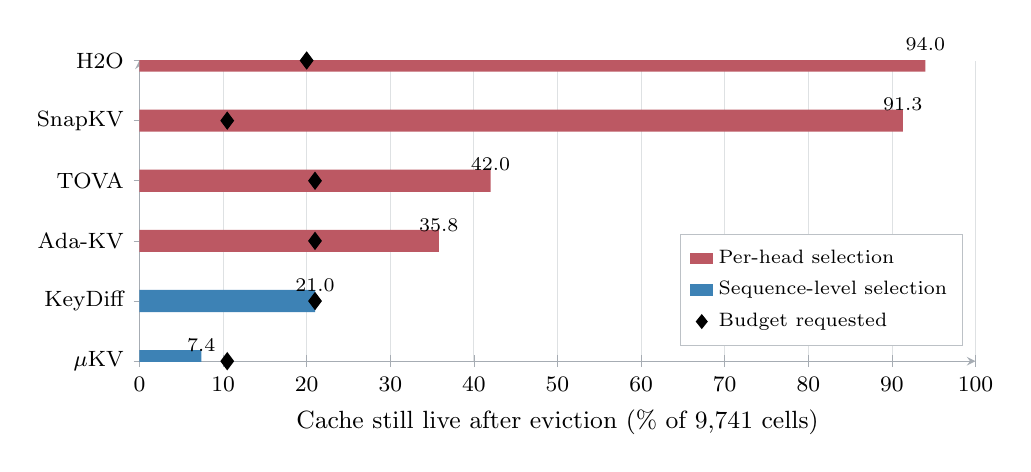
\begin{tikzpicture}
\begin{axis}[
  width=12.2cm, height=5.4cm, xbar, bar width=8pt,
  xmin=0, xmax=100, xlabel={Cache still live after eviction (\% of 9{,}741 cells)},
  symbolic y coords={muKV,KeyDiff,AdaKV,TOVA,SnapKV,H2O},
  ytick={muKV,KeyDiff,AdaKV,TOVA,SnapKV,H2O},
  yticklabels={$\mu$KV,KeyDiff,Ada-KV,TOVA,SnapKV,H2O},
  xmajorgrids, nodes near coords, nodes near coords style={font=\scriptsize},
  point meta=explicit symbolic, enlarge y limits=0.14, axis lines=left,
  legend style={at={(0.985,0.05)}, anchor=south east, draw=cG!45, fill=white,
                font=\scriptsize, cells={anchor=west}, row sep=1pt, inner sep=3.5pt},
  legend image post style={scale=0.85}]
\addplot[fill=cD!85,draw=none,bar shift=0pt,legend image code/.code={\draw[fill=cD!85,draw=none](0cm,-0.085cm) rectangle (0.34cm,0.085cm);}] coordinates {
  (94.0,H2O)[94.0] (91.3,SnapKV)[91.3] (42.0,TOVA)[42.0] (35.8,AdaKV)[35.8]};
\addlegendentry{Per-head selection}
\addplot[fill=cA!85,draw=none,bar shift=0pt,legend image code/.code={\draw[fill=cA!85,draw=none](0cm,-0.085cm) rectangle (0.34cm,0.085cm);}] coordinates {
  (21.0,KeyDiff)[21.0] (7.4,muKV)[7.4]};
\addlegendentry{Sequence-level selection}
\addlegendimage{only marks,mark=diamond*,mark size=3pt,fill=black,draw=black,legend image code/.code={\draw[fill=black,draw=black](0.17cm,0.10cm)--(0.25cm,0cm)--(0.17cm,-0.10cm)--(0.09cm,0cm)--cycle;}}
\addlegendentry{Budget requested}
\addplot[only marks,mark=diamond*,mark size=3pt,fill=black,draw=black,forget plot]
  coordinates {(20,H2O) (10.5,SnapKV) (21,TOVA) (21,AdaKV) (21,KeyDiff) (10.5,muKV)};
\end{axis}
\end{tikzpicture}
\\[10pt]
\textbf{\small (b) The same policy on two processors}\\[2pt]
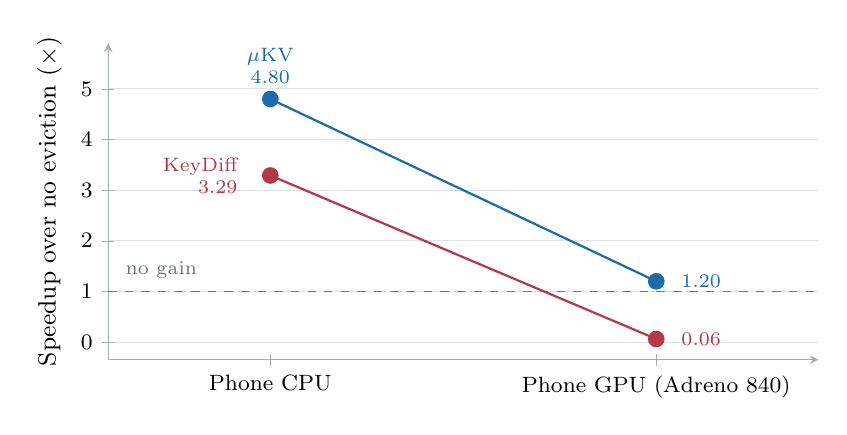
\begin{tikzpicture}
\begin{axis}[width=10.6cm,height=5.6cm,xmin=-.42,xmax=1.42,ymin=-0.35,ymax=5.9,
  xtick={0,1},xticklabels={Phone CPU,Phone GPU (Adreno 840)},
  ytick={0,1,2,3,4,5},
  ylabel={Speedup over no eviction ($\times$)},ymajorgrids,axis lines=left,
  clip=false]
\addplot[dashed,cG,forget plot] coordinates {(-.42,1)(1.42,1)};
\addplot[cA,thick,mark=*,mark size=2.6pt] coordinates {(0,4.80)(1,1.20)};
\addplot[cD,thick,mark=*,mark size=2.6pt] coordinates {(0,3.29)(1,0.06)};
\node[font=\scriptsize,cA,anchor=south,align=center] at (axis cs:0,4.92) {$\mu$KV\\4.80};
\node[font=\scriptsize,cA,anchor=west] at (axis cs:1.04,1.20) {1.20};
\node[font=\scriptsize,cD,anchor=east,align=right] at (axis cs:-0.06,3.29) {KeyDiff\\3.29};
\node[font=\scriptsize,cD,anchor=west] at (axis cs:1.04,0.06) {0.06};
\node[font=\scriptsize,cG,anchor=south west] at (axis cs:-0.40,1.06) {no gain};
\end{axis}
\end{tikzpicture}
\caption{\textbf{(a)} Per-head selection (red) keeps almost everything; sequence-level (blue)
gets its budget. Diamonds mark what was requested. \textbf{(b)} Llama-3.2-1B throughout, so
only the processor changes. The GPU point is a single run.}
\label{fig:findings}
\end{figure}

\subsection{The standard scoring route corrupts output on Adreno}
Reading attention weights requires an eval callback on the softmax node. A three-way control
on unmodified llama.cpp isolates the cause. Table~\ref{tab:control} gives it.

\begin{table}[h]\centering\small
\caption{The callback corrupts output even when it never reads the tensor, so the request is the trigger.}
\label{tab:control}
\begin{tabular}{@{}lr@{}}
\toprule
\textbf{Vanilla llama.cpp, FA off} & \textbf{Degenerate tokens}\\
\midrule
No callback & 0 / 978\\
Callback that reads the tensor & 76 / 609\\
\rowcolor{cA!8} Callback that requests but never reads & 68 / 679\\
\bottomrule
\end{tabular}
\end{table}

\noindent Requesting without reading corrupts equally, so the trigger is the request. In
\texttt{ggml\_backend\_}\allowbreak\texttt{sched\_compute\_splits}, a callback causes the backend split to be cut
into \texttt{ggml\_graph\_view} fragments, chunked where the callback is \emph{asked} for a
node, before any read. The same path is correct on the CPU backend (0.3\% degenerate across
271 cells, against 13.9\% across 607 on Adreno), so the scheduler design is not at fault. We
have not run a desktop-Vulkan control, so we do not separate llama.cpp's Vulkan code from the
Qualcomm driver.

\subsection{A hardware ceiling}
Each decoded token reads weights $W$ and live cache $KV$; eviction shrinks only $KV$, so
speedup cannot exceed $(W{+}KV)/W$. Table~\ref{tab:ceiling} evaluates it per model and processor.

\begin{table}[h]\centering\small
\caption{Eviction cannot beat the weight-bandwidth ceiling, and that ceiling belongs to the processor.}
\label{tab:ceiling}
\begin{tabular}{@{}lrrrr@{}}
\toprule
\textbf{Model and processor} & $W$ & $KV$ & \textbf{Ceiling} & \textbf{$\mu$KV reached}\\
\midrule
Llama-1B, phone GPU & 800\,MB & 319\,MB & $1.40\times$ & $1.20\times$\\
Phi-3-mini-128k, phone GPU & smaller & larger & $2.83\times$ & $2.64\times$\\
\rowcolor{cA!8} Llama-1B, phone CPU & \multicolumn{2}{c}{not the limit} & none & $4.80\times$\\
\bottomrule
\end{tabular}
\end{table}

\noindent The ceiling assumes decode waits on weight bytes. On the CPU it waits on attention
arithmetic over live cells, so shrinking cells shrinks work directly. The strongest evidence
is a baseline, not our design.



\paragraph{How firm the ceiling is.} The bound is analytical and no measured policy exceeded
it. It is not what binds on this GPU: $\mu$KV retains 7.4\% and StreamingLLM 20.6\%, a
$2.8\times$ difference, and both reach $1.20\times$ where the roofline predicts $1.36\times$
and $1.29\times$. Observed speedup is flat in retention, which strengthens the deployment
conclusion: on this GPU, freeing $2.8\times$ more cache buys nothing.

\section{Design}
$\mu$KV is not offered as a better eviction rule (Fig.~\ref{fig:arch}). It is what the three findings force.

\begin{figure}[h]\centering
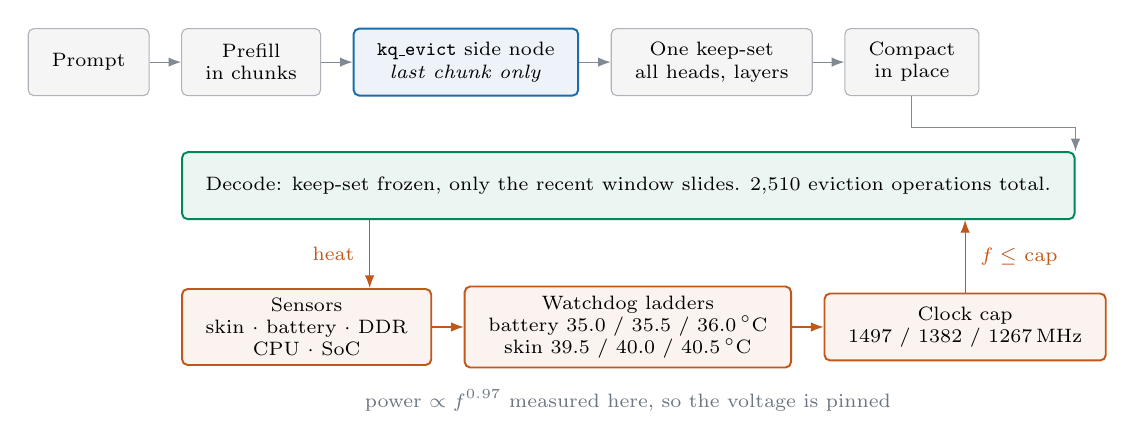
\begin{tikzpicture}[
  node distance=4mm, font=\scriptsize,
  bx/.style={draw=cG!55,fill=cG!7,rounded corners=2pt,minimum height=8.5mm,inner xsep=3mm,align=center},
  hi/.style={bx,draw=cA,fill=cA!8,line width=.7pt},
  gn/.style={bx,draw=cC,fill=cC!8,line width=.7pt},
  th/.style={bx,draw=cB,fill=cB!7,line width=.7pt},
  ar/.style={-{Latex[length=1.6mm]},cG!85}]
\node[bx] (p) {Prompt};
\node[bx,right=of p] (pf) {Prefill\\in chunks};
\node[hi,right=of pf] (sn) {\texttt{kq\_evict} side node\\\emph{last chunk only}};
\node[bx,right=of sn] (ks) {One keep-set\\all heads, layers};
\node[bx,right=of ks] (cp) {Compact\\in place};
\draw[ar](p)--(pf); \draw[ar](pf)--(sn); \draw[ar](sn)--(ks); \draw[ar](ks)--(cp);
\node[gn,below=7mm of pf.south west,anchor=north west,minimum width=9.1cm] (dec)
  {Decode: keep-set frozen, only the recent window slides. 2{,}510 eviction operations total.};
\draw[ar] (cp.south) |- ([yshift=3mm]dec.north east) -- (dec.north east);
\node[th,below=13mm of dec.west,anchor=north west] (t1)
  {Sensors\\skin $\cdot$ battery $\cdot$ DDR\\CPU $\cdot$ SoC};
\node[th,right=of t1] (t2)
  {Watchdog ladders\\battery 35.0 / 35.5 / 36.0\,$^\circ$C\\skin 39.5 / 40.0 / 40.5\,$^\circ$C};
\node[th,right=of t2] (t3) {Clock cap\\1497 / 1382 / 1267\,MHz};
\draw[-{Latex[length=1.6mm]},cB](t1)--(t2);
\draw[-{Latex[length=1.6mm]},cB](t2)--(t3);
% the loop closes THROUGH decode: the clock cap is what decode runs under
\draw[-{Latex[length=1.6mm]},cB] ([xshift=8mm]dec.south -| t1) -- ([xshift=8mm]t1.north)
  node[midway,left=2pt,font=\scriptsize,cB] {heat};
\draw[-{Latex[length=1.6mm]},cB] (t3.north) -- (dec.south -| t3)
  node[midway,right=2pt,font=\scriptsize,cB] {$f \le$ cap};
\node[below=1.5mm of t2,font=\scriptsize,cG]
  {power $\propto f^{0.97}$ measured here, so the voltage is pinned};
\end{tikzpicture}
\caption{In-graph scoring answers \S3.2; one keep-set answers \S3.1. The loop closes through
decode: work makes heat, the watchdog reads five sensors, and the clock cap it sets is what
decode runs under.}
\label{fig:arch}
\end{figure}

\begin{table}[h]\centering\small
\caption{Where each class sits. All four evict from the same shared cell array; what differs
is the signal each reads and whether it selects before or after aggregating over heads. The
last two columns summarise Table~\ref{tab:niah}.}
\label{tab:classes}
\begin{tabular}{@{}llccccr@{}}
\toprule
\textbf{Class} & \textbf{Policies} & \textbf{Signal} & \textbf{FA} &
\textbf{Seq.} & \textbf{NIAH} & \textbf{Kept}\\
\midrule
per-head        & SnapKV, Ada-KV,      & attention    & off & no  & 2--12/14 & 52--99\%\\
                & H2O, TOVA            & scores       &     &     &          &         \\
position-blind  & StreamingLLM         & none         & on  & yes & 7/14     & 32.9\%\\
key-geometry    & KeyDiff              & key          & on  & yes & 14/14    & 33.6\%\\
                &                      & similarity   &     &     &          &         \\
\rowcolor{cA!8} attention-scored & $\mu$KV & attention mass, & on & yes & \textbf{14/14} & \textbf{13.0\%}\\
\rowcolor{cA!8}                  &         & in graph        &    &     &                &        \\
\bottomrule
\end{tabular}
\end{table}

\noindent Table~\ref{tab:classes} places every class. Only the sequence-level classes compact, and that is the whole of the realizability
gap: a head may nominate a position, but only a sequence-level policy decides one. KeyDiff and
$\mu$KV share the outcome column and differ in the signal, which is what separates 33.6\% from
13.0\% at the same 14/14.

\paragraph{How it is attention-scored while FlashAttention stays on.} It does not read
anything out of FlashAttention. FlashAttention never writes its scores, so instead the side
node computes its own $\mathrm{softmax}(\text{kq\_scale}\cdot K^{\top}Q_{\text{last }W})$
beside it, which is the same arithmetic the FA-off path would have produced. The saving is
that it does this for the last $W{=}16$ query rows only, not for all $N$. On a 9{,}737-token
prompt that is a $16\times N$ matrix instead of $N\times N$, about 0.16\% of the full
attention, which is why prefill moves $+0.7\%$ rather than the $+33$ to $+111\%$ that turning
FlashAttention off costs.

The scores are then averaged over those $W$ queries \emph{on the device}
(\texttt{sum\_rows}$/W$), so the host reads one number per position per head rather than $W$ of
them, and the transfer is $W$ times smaller. It runs on the last prefill chunk only. So the
signal is genuine attention mass, not a proxy for it, and the main attention path is never
disturbed.

\paragraph{Why a per-head gate inside a sequence-level policy.} The gate really is per head,
and it does more than score: it selects. It reads each head's own peak attention $\max a_h$,
gives that head its own budget $K_h$, and takes that head's top-$K_h$ positions. What it does
not do is decide eviction. Those sets are unioned over the heads in a layer and again over
layers, and the union is only a candidate pool.

Exactly three things in $\mu$KV are per head: the statistic $\max a_h$, the budget $K_h$, and
that head's top-$K_h$ pick. Everything after that is sequence-level. The position scores are
$\bar a_p$, summed over every layer and head and divided by their count, so one number per
position. The $\alpha$-gate reads that averaged vector, not any head. The anchor and recent
split, the four sink positions, the 1D pooling and the final top-$K$ all operate on the
sequence. So a head can nominate a position, but no head can keep one.

That union is the same operation that defeats SnapKV and AhaKV in \S3.1. Here it is harmless,
because it produces only a candidate pool and a single global top-$K$ caps the result at $K$.
In a per-head method the union \emph{is} the answer, so nothing bounds it, which is why SnapKV
asks for 1024 cells and keeps 8893. $\mu$KV is sequence-level in what it emits, not in how it
scores.

\paragraph{Where each part comes from.} No box in that figure is new on its own, and we do not
claim otherwise. Scoring inside an observation window and pooling the position scores with a 1D
kernel are SnapKV's~\cite{snapkv}. Sizing each head's share from its own attention
concentration is Ada-KV's idea~\cite{adakv}. Selecting at sequence level while FlashAttention
stays on is KeyDiff's~\cite{keydiff}. Computing an eviction score alongside self-attention
rather than from the attention matrix is AhaKV's~\cite{ahakv}. Keeping a few sink tokens is
StreamingLLM's~\cite{streamingllm}.

The arrangement is another matter. We have not found this pipeline in any single paper:
attention mass taken from inside the FlashAttention graph, pooled, gated per head but emitted
as \emph{one} keep-set for all heads and layers, then compacted so the drop is physical. AhaKV
has the scoring signal but selects per head. KeyDiff emits one set but scores on key geometry.
Neither compacts. Our search was by keyword rather than exhaustive, so we state this as what we
could not find, not as a proof that it does not exist.

The arrangement is also not arbitrary. Each choice answers one of the three findings in \S3,
and the result is measurable rather than merely different: $\mu$KV reaches 14/14 retrieval on
13.0\% of the cache where KeyDiff needs 33.6\%. That is the scoring signal earning its place,
not a relabelling of parts.

Compaction is not ours either. llama.cpp shipped a KV defragmenter, now deprecated and removed;
prior work reports contiguous compaction with a measured per-step cost; and vLLM and SGLang
reach the same end by paging or by remapping virtual memory. What we add there is an
\emph{in-place} slide that needs no second context, where the state round-trip is killed by the
OS at 16K, verified byte-identical on 23 of 25 pairs, and shown to be the precondition for
handing pages back.

So this is a composition claim, and a composition is weaker than a new mechanism. But one
forced by measured constraints and validated on quality per retained cell is a contribution
rather than a rearrangement, and it sits alongside the measurement in \S3 and \S6 rather than
beneath it.

\begin{figure}[h]\centering
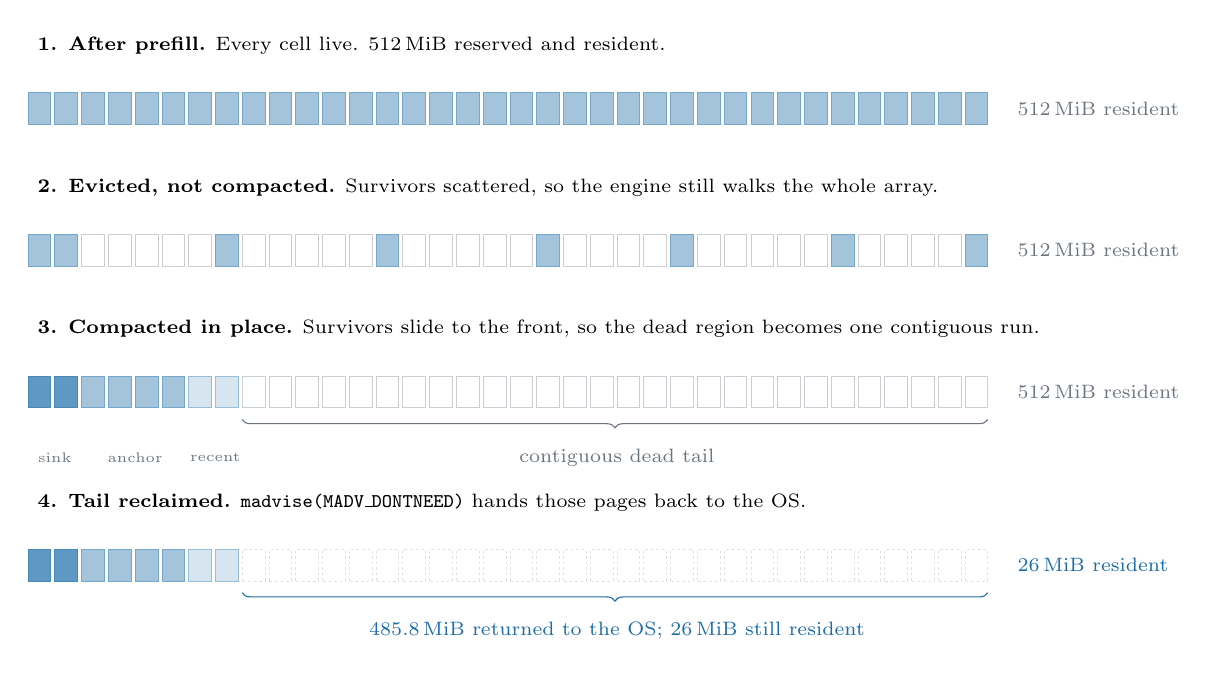
\begin{tikzpicture}[x=3.4mm,y=1mm,font=\scriptsize]
\def\N{36}
% --- row 1: after prefill ---
\node[anchor=west,font=\scriptsize,cG] at (36.6,2)   {512\,MiB resident};
\node[anchor=west,font=\scriptsize,cG] at (36.6,-16) {512\,MiB resident};
\node[anchor=west,font=\scriptsize,cG] at (36.6,-34) {512\,MiB resident};
\node[anchor=west,font=\scriptsize,cA] at (36.6,-56) {26\,MiB resident};
\node[anchor=west,align=left] at (0,10) {\textbf{1. After prefill.} Every cell live. 512\,MiB reserved and resident.};
\foreach \i in {0,...,35}{\draw[fill=cA!40,draw=cA!60,line width=.2pt] (\i,0) rectangle ++(0.85,4);}
% --- row 2: evicted, not compacted ---
\node[anchor=west,align=left] at (0,-8) {\textbf{2. Evicted, not compacted.} Survivors scattered, so the engine still walks the whole array.};
\foreach \i in {0,...,35}{\draw[draw=cG!35,line width=.2pt] (\i,-18) rectangle ++(0.85,4);}
\foreach \i in {0,1,7,13,19,24,30,35}{\draw[fill=cA!40,draw=cA!60,line width=.2pt] (\i,-18) rectangle ++(0.85,4);}
% --- row 3: compacted ---
\node[anchor=west,align=left] at (0,-26) {\textbf{3. Compacted in place.} Survivors slide to the front, so the dead region becomes one contiguous run.};
\foreach \i in {0,...,35}{\draw[draw=cG!35,line width=.2pt] (\i,-36) rectangle ++(0.85,4);}
\foreach \i in {0,1}{\draw[fill=cA!70,draw=cA!80,line width=.2pt] (\i,-36) rectangle ++(0.85,4);}
\foreach \i in {2,...,5}{\draw[fill=cA!40,draw=cA!60,line width=.2pt] (\i,-36) rectangle ++(0.85,4);}
\foreach \i in {6,7}{\draw[fill=cA!18,draw=cA!45,line width=.2pt] (\i,-36) rectangle ++(0.85,4);}
\node[anchor=north,font=\tiny,cG] at (1,-40.5) {sink};
\node[anchor=north,font=\tiny,cG] at (4,-40.5) {anchor};
\node[anchor=north,font=\tiny,cG] at (7,-40.5) {recent};
\draw[decorate,decoration={brace,amplitude=3pt},cG] (35.85,-37.5) -- (8,-37.5);
\node[anchor=north,cG] at (22,-40) {contiguous dead tail};
% --- row 4: reclaimed ---
\node[anchor=west,align=left] at (0,-48) {\textbf{4. Tail reclaimed.} \texttt{madvise(MADV\_DONTNEED)} hands those pages back to the OS.};
\foreach \i in {0,1}{\draw[fill=cA!70,draw=cA!80,line width=.2pt] (\i,-58) rectangle ++(0.85,4);}
\foreach \i in {2,...,5}{\draw[fill=cA!40,draw=cA!60,line width=.2pt] (\i,-58) rectangle ++(0.85,4);}
\foreach \i in {6,7}{\draw[fill=cA!18,draw=cA!45,line width=.2pt] (\i,-58) rectangle ++(0.85,4);}
\foreach \i in {8,...,35}{\draw[draw=cG!22,line width=.2pt,dash pattern=on 1pt off 1pt] (\i,-58) rectangle ++(0.85,4);}
\draw[decorate,decoration={brace,amplitude=3pt},cA] (35.85,-59.5) -- (8,-59.5);
\node[anchor=north,cA] at (22,-62) {485.8\,MiB returned to the OS; 26\,MiB still resident};
\end{tikzpicture}
\caption{Resident memory is unchanged through steps 1 to 3: neither eviction nor compaction
frees anything. Only step 4 does, and only because step 3 made the run contiguous.}
\label{fig:memstates}
\end{figure}

\begin{enumerate}\itemsep1pt\parskip0pt
\item \textbf{Score inside the graph.} A \texttt{kq\_evict} side node makes scores something
the graph produces. No callback, and FlashAttention never turns off. Answers \S3.2.
\item \textbf{One keep-set, packed.} A single keep-set for all heads and layers; survivors
slide into a contiguous prefix. Answers \S3.1.
\item \textbf{Freeze during decode.} The keep-set is chosen once at the end of prefill; only
the recent window slides, so scoring costs nothing per token.
\item \textbf{Compact in place.} Survivors slide inside the existing tensors. The state
round-trip alternative needs a second full context and is killed by the OS at 16K.
\end{enumerate}

\subsection{Comparison with KeyDiff}
KeyDiff also selects at sequence level and evicts with FlashAttention on, so it avoids \S3.1
as well. We claim no priority on eviction itself. Table~\ref{tab:keydiff} isolates what does differ.

\begin{table}[h]\centering\small
\caption{What separates $\mu$KV from KeyDiff, restricted to what no other table here already
gives. Budgets, throughput and retention are in Tables~\ref{tab:cpu} and~\ref{tab:niah}.}
\label{tab:keydiff}
\begin{tabular}{@{}lrr@{}}
\toprule
\textbf{Llama-1B, phone CPU, same campaign} & \textbf{$\mu$KV} & \textbf{KeyDiff}\\
\midrule
\rowcolor{cA!8} Eviction operations during decode & 2{,}510 & 59{,}238\\
Peak RSS above vanilla & $+12$ to $+126$\,MiB & $+0$\,MiB\\
Thermal governor & yes & none\\
\bottomrule
\end{tabular}
\end{table}

\noindent $\mu$KV fixes the keep-set once; KeyDiff re-evicts block-wise throughout
generation, $24\times$ more work. That is why it is slower on the CPU in the same class, and
why it inverts on the GPU where each eviction costs more than the smaller cache saves.
Because $\mu$KV scores on attention mass rather than key geometry, it reaches the same 14/14
retrieval on 13.0\% of the cache where KeyDiff needs 33.6\%. Compaction and the thermal loop
are ours; neither is part of KeyDiff.

\section{Experimental design}
OnePlus 15, Snapdragon 8 Elite Gen 5, Adreno 840; llama.cpp, one build per table; f16 KV
throughout, since q8\_0 is numerically broken on this Adreno driver. Four models:
Llama-3.2-1B Q4\_K\_M, Phi-3-mini-128k Q4\_K\_M, Bonsai-8B Q1\_0 (1-bit), gemma-2-2b
(interleaved sliding-window attention). Nine policies, each at its own published
configuration, never forced to a common budget. Benchmarks: WikiText (9.7K prompt, 4K
decode), needle-in-a-haystack (14 stimuli $\times$ 7 depths), LongBench token-F1.

\paragraph{Measurement discipline.}
Cool gate before every timed cell (DDR $\le$ 35\,$^\circ$C, battery $\le$ 33\,$^\circ$C,
cores $\le$ 45\,$^\circ$C, charging off). Scheduler pinning, because unpinned identical GPU
runs spread 28.2--39.2 tok/s; pinning collapses that to 3\%. $n{=}3$ with Latin-square
rotation on every headline row. Energy from the USB rail and the coulomb counter. Text graded
for degeneracy before any timing is quoted. Clock pinning at 1632\,MHz for the prefill study,
adopted only after four attempts to control temperature instead had failed.

\section{Evaluation}
\subsection{Sustained decode, phone CPU}
Table~\ref{tab:cpu} is the headline campaign, and Fig.~\ref{fig:tps} plots it against the cache each policy actually freed.
\begin{table}[h]\centering\small
\caption{Llama-3.2-1B Q4\_K\_M, 6 threads, 9.7K prompt and 4096 decoded tokens.}
\label{tab:cpu}
\begin{tabular}{@{}llrrrrr@{}}
\toprule
\textbf{Policy} & \textbf{Config} & \textbf{tok/s} & \textbf{$\times$van} &
\textbf{Wall (s)} & \textbf{mWh} & \textbf{Live cells}\\
\midrule
\rowcolor{cA!8} $\mu$KV & $K{=}1024$ & 23.91\,$\pm$0.37 & 4.80 & 379 & 595 & 721\\
KeyDiff & $K{=}2048$ & 16.40\,$\pm$0.11 & 3.29 & 484 & 700 & 2049\\
Ada-KV & FA on & 11.52 & 2.29 & 566 & 845 & 3489\\
StreamingLLM & 4+2000 & 10.25\,$\pm$0.06 & 2.06 & 580 & 781 & 2001\\
SnapKV & FA off & 6.83 & 1.36 & 849 & 1180 & 5931\\
Ada-KV & FA off & 6.79 & 1.35 & 856 & 1194 & 3485\\
H2O & FA off & 6.45 & 1.29 & 856 & 1262 & \textit{9151}\\
KeyDiff & $K{=}8192$ & 6.43 & 1.28 & 812 & 1261 & 8195\\
TOVA & FA off & 5.92 & 1.18 & 917 & 1200 & 4093\\
SnapKV & FA on & 5.38 & 1.07 & 953 & 1346 & \textit{8893}\\
vanilla & full cache & 4.99\,$\pm$0.01 & 1.00 & 1004 & 1431 & 9741\\
\bottomrule
\end{tabular}
\end{table}

\begin{figure}[h]\centering
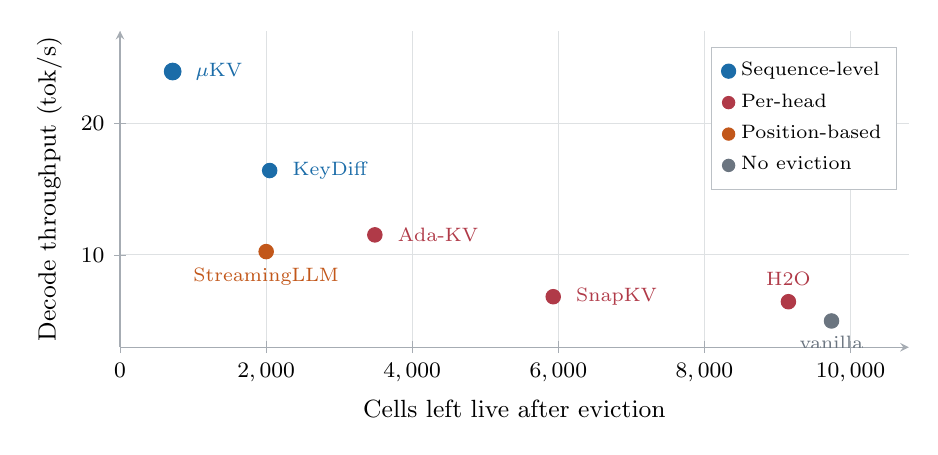
\begin{tikzpicture}
\begin{axis}[width=11.6cm,height=5.6cm,
  xlabel={Cells left live after eviction}, ylabel={Decode throughput (tok/s)},
  xmin=0,xmax=10800,ymin=3,ymax=27,grid=both,axis lines=left,
  scaled x ticks=false, xtick={0,2000,4000,6000,8000,10000},
  x tick label style={/pgf/number format/1000 sep={,}},
  legend style={at={(0.985,0.95)}, anchor=north east, draw=cG!45, fill=white,
                font=\scriptsize, cells={anchor=west}, row sep=1pt, inner sep=3.5pt},
  legend image post style={scale=0.85},
  every node near coord/.append style={font=\scriptsize,anchor=west,xshift=2pt}]
\addplot[only marks,mark=*,mark size=3pt,cA] coordinates {(721,23.91)};
\addlegendentry{Sequence-level}
\addplot[only marks,mark=*,mark size=2.6pt,cD] coordinates {(9151,6.45)};
\addlegendentry{Per-head}
\addplot[only marks,mark=*,mark size=2.6pt,cB] coordinates {(2001,10.25)};
\addlegendentry{Position-based}
\addplot[only marks,mark=*,mark size=2.6pt,cG] coordinates {(9741,4.99)};
\addlegendentry{No eviction}
\addplot[only marks,mark=*,mark size=2.6pt,cA,forget plot] coordinates {(2049,16.40)};
\addplot[only marks,mark=*,mark size=2.6pt,cD,forget plot] coordinates {(3489,11.52)(5931,6.83)};
\node[font=\scriptsize,cA,anchor=west]  at (axis cs:900,23.91)  {$\mu$KV};
\node[font=\scriptsize,cA,anchor=west]  at (axis cs:2230,16.40) {KeyDiff};
\node[font=\scriptsize,cD,anchor=west]  at (axis cs:3670,11.52) {Ada-KV};
\node[font=\scriptsize,cB,anchor=north] at (axis cs:2001,9.75)  {StreamingLLM};
\node[font=\scriptsize,cD,anchor=west]  at (axis cs:6110,6.83)  {SnapKV};
\node[font=\scriptsize,cD,anchor=south] at (axis cs:9151,6.95)  {H2O};
\node[font=\scriptsize,cG,anchor=north] at (axis cs:9741,4.55)  {vanilla};
\end{axis}
\end{tikzpicture}
\caption{Throughput tracks cells actually freed, not the budget requested. StreamingLLM is
the outlier because it keeps by position rather than by evidence.}
\label{fig:tps}
\end{figure}

\subsection{Retrieval and quality}
Table~\ref{tab:niah} covers retrieval and Table~\ref{tab:longbench} the LongBench scores.
\begin{table}[h]\centering\small
\caption{Needle retrieval on the phone GPU, read against the cache each policy kept at 4K and
8K depth.}
\label{tab:niah}
\begin{tabular}{@{}lrrrr@{}}
\toprule
\textbf{Needle, GPU} & $K$ & \textbf{Found} & \multicolumn{2}{c}{\textbf{Kept 4K / 8K}}\\
\midrule
vanilla                 & ---  & 14/14 & 100\%  & 100\%\\
\rowcolor{cA!8} $\mu$KV & 1024 & 14/14 & 25.2\% & 13.0\%\\
KeyDiff                 & 2048 & 14/14 & 65.6\% & 33.6\%\\
KeyDiff                 & 6144 & 14/14 & 100\%  & 100\%\\
Ada-KV                  & 1024 & 12/14 & 76.9\% & 52.2\%\\
SnapKV                  & 1024 & 12/14 & 100\%  & 98.2\%\\
StreamingLLM            & 2004 & 7/14  & 64.2\% & 32.9\%\\
H2O                     & 1024 & 3/14  & 100\%  & 99.3\%\\
TOVA                    & 1024 & 2/14  & 85.2\% & 60.7\%\\
\bottomrule
\end{tabular}
\end{table}

\begin{table}[h]\centering\small
\caption{Every policy with hotpotqa data, on the 15 indices all of them share. Read F1
against retention: the four above vanilla all keep 54--92\% of the cache, and three of them
beat the full cache, which is impossible and is the tell for noise at this sample size.}
\label{tab:longbench}
\begin{tabular}{@{}lrr@{}}
\toprule
\textbf{LongBench, hotpotqa} & \textbf{F1} & \textbf{Kept}\\
\midrule
Ada-KV                 & 40.00 & 53.6\%\\
SnapKV                 & 40.00 & 88.8\%\\
TOVA                   & 39.89 & 57.2\%\\
H2O                    & 39.79 & 91.6\%\\
KeyDiff 8K             & 36.39 & 62.2\%\\
vanilla                & 36.00 & 99.8\%\\
\rowcolor{cA!8} $\mu$KV & 29.79 & 13.6\%\\
KeyDiff 6K             & 29.33 & 48.3\%\\
StreamingLLM           & 23.57 & 19.4\%\\
KeyDiff 2K             & 15.84 & 20.0\%\\
\bottomrule
\end{tabular}
\end{table}

\noindent $\mu$KV also reaches 14/14 on the CPU backend for Phi-3 (17\% retained) and
Bonsai-8B (18\%). \textbf{Limit of the F1 table:} at $n{=}15$ a single question moves the
score by 6.7 points. $\mu$KV and the full cache answer 13 of 15 identically, one win and one
loss each way, sign-test $p{=}1.00$. Every standard error (6.5--12.0 F1) exceeds every gap in
the table. Retention separates these policies at this sample size; F1 does not.

\subsection{Accuracy against budget}
Every table so far reports one budget per policy, which shows a point and not a curve. Running
$\mu$KV on Bonsai-8B at $K=1024$, $2048$ and $4096$ gives the shape.

\begin{figure}[h]\centering
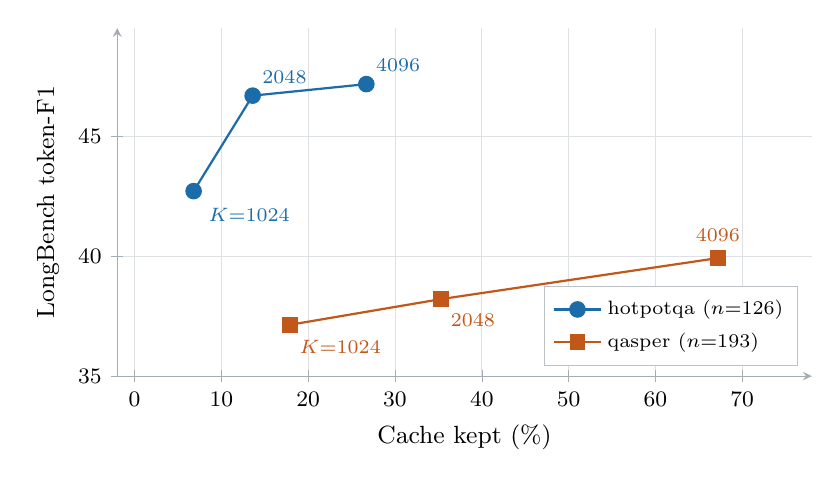
\begin{tikzpicture}
\begin{axis}[width=10.4cm,height=6cm,
  xlabel={Cache kept (\%)}, ylabel={LongBench token-F1},
  xmin=-2,xmax=78,ymin=35,ymax=49.5,grid=both,axis lines=left,
  legend style={at={(0.98,0.03)},anchor=south east,draw=cG!45,fill=white,
                font=\scriptsize,cells={anchor=west},row sep=1pt,inner sep=3pt},
  every node near coord/.append style={font=\scriptsize,anchor=south,yshift=1pt}]
\addplot[cA,thick,mark=*,mark size=2.6pt,nodes near coords={\phantom{x}}]
  coordinates {(6.8,42.71) (13.6,46.69) (26.7,47.17)};
\addlegendentry{hotpotqa ($n{=}126$)}
\addplot[cB,thick,mark=square*,mark size=2.4pt]
  coordinates {(17.9,37.14) (35.3,38.21) (67.2,39.92)};
\addlegendentry{qasper ($n{=}193$)}
\node[font=\scriptsize,cA,anchor=north west] at (axis cs:7.4,42.4) {$K{=}1024$};
\node[font=\scriptsize,cA,anchor=south west] at (axis cs:13.6,46.8) {2048};
\node[font=\scriptsize,cA,anchor=south west] at (axis cs:26.7,47.3) {4096};
\node[font=\scriptsize,cB,anchor=north west] at (axis cs:17.9,36.9) {$K{=}1024$};
\node[font=\scriptsize,cB,anchor=north west] at (axis cs:35.3,38.0) {2048};
\node[font=\scriptsize,cB,anchor=south] at (axis cs:67.2,40.2) {4096};
\end{axis}
\end{tikzpicture}
\caption{Both tasks are monotone in budget, and both bend early. Scored on the indices all
three budgets share, so the three points compare like for like.}
\label{fig:budget}
\end{figure}

\noindent The knee is sharp on hotpotqa. Going from $K{=}1024$ to $2048$ costs 6.8 more points
of cache and buys 3.98\,F1; going on to 4096 costs another 13.1 points of cache and buys
0.48\,F1. Quadrupling the budget from 1024 to 4096 buys 4.46\,F1 in total, so $K{=}1024$
already holds 91\% of the quality available at four times the cache. qasper is flatter still:
67.2\% retention scores 39.92 against 37.14 at 17.9\%, which is 2.78\,F1 for nearly four times
the cache.

That is the argument for a fixed, small $K$ rather than a generous one, and it is also why the
energy-aware controller in \S8 should modulate $K$ over a narrow band near the knee rather
than across the whole range.

\subsection{Compaction, and returning memory to the OS}
Table~\ref{tab:compact} separates the two, Fig.~\ref{fig:memstates} shows the four memory states, and Fig.~\ref{fig:rss} the resident totals.
\begin{table}[h]\centering\small
\caption{Compaction changes bytes read per token, not peak allocation.}
\label{tab:compact}
\begin{tabular}{@{}lrrr@{}}
\toprule
\textbf{Llama-1B, phone GPU} & \textbf{vanilla} & \textbf{$\mu$KV} & \textbf{Change}\\
\midrule
Peak cache allocated & 432\,MB & 392\,MB & $-9\%$\\
\rowcolor{cA!8} Cache read per token & 304\,MB & 23\,MB & $-93\%$\\
\bottomrule
\end{tabular}
\end{table}

\noindent The engine reserves the full context up front, so peak memory barely moves. The
gain is bandwidth, and the paper says so rather than claiming a memory saving.

\paragraph{New result (31 August 2026).} The cache is one buffer sized for the full context,
and setup ends with \texttt{ggml\_backend\_buffer\_clear}, which writes zero to every page.
Residency is therefore fixed at allocation: 512\,MiB resident before a single token exists.
No policy can change that. Compaction makes the fix possible, because once survivors slide to
the front the dead cells are contiguous and their pages can be released with
\texttt{madvise(MADV\_DONTNEED)} while the mapping stays. We implemented this in llama.cpp
(32 calls, one per K and V tensor) and measured it on device.

The 485.8\,MiB recovered is close to the arithmetic maximum, not a partial result. The buffer
holds 16{,}384 cells at 32\,KiB each, or 512\,MiB. After eviction 837 cells are live, so 15{,}547
are dead and the most that can be freed is 485.8\,MiB; we free 99.98\% of that, the remainder
being page rounding across the 32 regions. The recovered share of the buffer (94.9\%) is larger
than the share evicted from the prompt (89\%) because the buffer is sized for the full 16K
context while the prompt used only 7{,}755 cells. Those extra cells were never read by anything,
but the init memset made them resident, so they are recovered too.

\begin{figure}[h]\centering
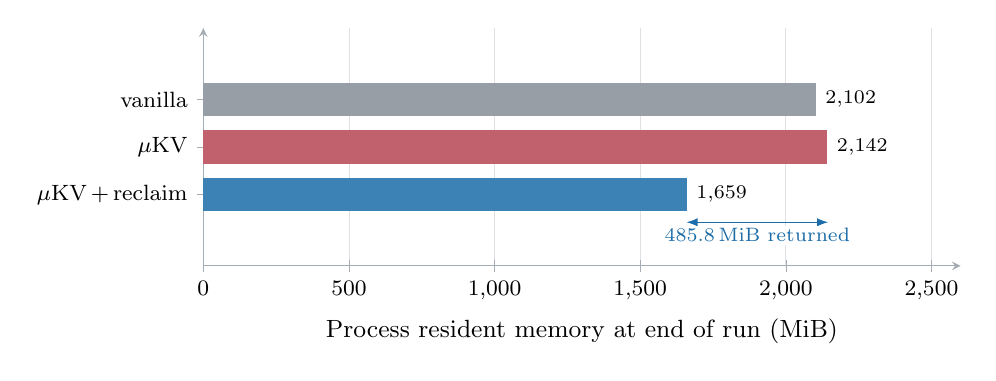
\begin{tikzpicture}
\begin{axis}[width=11.2cm,height=4.6cm,xbar,bar width=12pt,
  xmin=0,xmax=2600,xlabel={Process resident memory at end of run (MiB)},
  symbolic y coords={rec,mu,van},
  ytick={van,mu,rec},
  yticklabels={vanilla,$\mu$KV,$\mu$KV\,+\,reclaim},
  xtick={0,500,1000,1500,2000,2500},
  xmajorgrids,axis lines=left,nodes near coords,
  nodes near coords style={font=\scriptsize},enlarge y limits=0.75,clip=false]
\addplot[fill=cG!70,draw=none,bar shift=0pt] coordinates {(2102,van)};
\addplot[fill=cD!80,draw=none,bar shift=0pt] coordinates {(2142,mu)};
\addplot[fill=cA!85,draw=none,bar shift=0pt] coordinates {(1659,rec)};
\draw[{Latex[length=1.4mm]}-{Latex[length=1.4mm]},cA]
  ([yshift=-10pt]axis cs:1659,rec) -- ([yshift=-10pt]axis cs:2145,rec);
\node[font=\scriptsize,cA,anchor=north,fill=white,inner sep=1pt]
  at ([yshift=-11pt]axis cs:1902,rec) {485.8\,MiB returned};
\end{axis}
\end{tikzpicture}
\caption{Llama-3.2-1B, phone CPU, 16K context. Text is byte-identical with and without the
reclaim and throughput does not fall. Peak RSS is unchanged: the init memset sets it.}
\label{fig:rss}
\end{figure}

\noindent\textbf{Why $\mu$KV sits above vanilla in that figure.} The \texttt{kq\_evict} side
node adds graph tensors sized by $n_{kv}$, so llama.cpp reallocates the compute buffer past its
worst-case reservation, 32.3 to 58.2\,MiB on a 9.4K prompt. Because those tensors scale with
the prompt, so does the overhead.

$\mu$KV alone uses more memory than vanilla, and the overhead grows with the prompt. The side
node adds graph tensors sized by $n_{kv}$, so llama.cpp reallocates the compute buffer past its
worst-case reservation, 32.3 to 58.2\,MiB on a 9.4K prompt. Measured across 30 prompt lengths
in one campaign, peak RSS runs $+12$\,MiB above vanilla at 2.2K tokens and $+126$\,MiB at
16.3K. With reclaim the run ends 444\,MiB below vanilla at 25.71 against 25.22 tok/s.

The comparison with KeyDiff is unflattering here and worth stating. In the same campaign
KeyDiff's peak RSS matches vanilla to within 1\,MiB at every one of those 30 lengths, because
it scores on key geometry read host-side and adds no graph tensors. It also bounds the live
cache from the first block, where $\mu$KV holds the whole prompt until the end of prefill. So
on memory during prefill KeyDiff is strictly better, and the per-head policies are strictly
worse than both: SnapKV runs $+31$ to $+282$\,MiB over vanilla and H2O $+47$ to $+376$.

\subsection{What $\mu$KV delivers}
Three claims. Each is stated with its evidence and its limit.

\textbf{Energy: yes.} The same 4096 tokens cost 595\,mWh against vanilla's 1431\,mWh on the
phone CPU, which is 58\% less. This is the strongest of the three.

\textbf{Memory: only with the tail reclaim.} The shipped design does not save memory. It uses
40\,MiB \emph{more} than vanilla, because the scoring side node enlarges the compute buffer.
Adding the reclaim returns 485.8\,MiB and ends the run 444\,MiB below vanilla. That result is
one model, one prompt, $n{=}1$, and new code, so it is a demonstrated follow-on, not a
shipped property.

\textbf{Sustained speed: from efficiency, not from the watchdog.} $\mu$KV holds about
23.1\,tok/s flat across a 42-minute soak, and the watchdog is not what does it. With the
watchdog off $\mu$KV already sustains 23.14\,tok/s. With it on, later generations run
22.97\,tok/s, which is 0.8\% slower. The gain is confined to the first generation, $+15.5\%$,
after which both arms settle at the same clock: 1382 against 1383\,MHz. The watchdog does not
prevent the vendor cliff either, since every arm still touches 883\,MHz. What it does change
is time spent deeply throttled, 21.8\% of samples below 1200\,MHz with it off against 17.5\%
with it on, and that reduction does not turn into throughput. The watchdog is a front-loaded
dial, not a way to hold the clock up.

\textbf{Clock and power, and why the ladder is a weak lever.} Raising the clock does raise
power, but in proportion, not as the cube. We swept the prime core across five frequencies, two repeats each (Table~\ref{tab:power}). Power came from the USB
rail with charging disabled, so the battery neither drew nor supplied anything and the rail
carried the whole device.

\begin{table}[h]\centering\small
\caption{Prime-core frequency against system power. The relation is linear, not cubic.}
\label{tab:power}
\begin{tabular}{@{}rrrr@{}}
\toprule
\textbf{Clock (MHz)} & \textbf{System power (W)} & \textbf{Dynamic part (W)} & \textbf{tok/s}\\
\midrule
883  & 2.29 & 2.04 & 7.36\\
1018 & 2.48 & 2.23 & 8.31\\
1267 & 2.98 & 2.74 & 10.27\\
1498 & 3.53 & 3.28 & 11.83\\
1632 & 3.97 & 3.72 & 13.44\\
\bottomrule
\end{tabular}
\end{table}

A straight line fits these points with $R^2=0.99$: power is $0.25\,\mathrm{W} + 2.23\,\mathrm{mW}$
per MHz. Removing that 0.25\,W static floor leaves a dynamic part that scales as $f^{0.97}$,
which is linear to within measurement error.

This matters for the design. Dynamic power is $C V^2 f$. It falls as the cube of the clock
only when the voltage is lowered along with the frequency. An exponent of 1 means the voltage
did not move at all across 883 to 1632\,MHz, so the governor was changing frequency at a fixed
voltage. We could not read the core voltage directly on this device, so the exponent is our
evidence for it.

The consequence is that the clock ladder is a weak thermal lever by construction. One step
down, 1497 to 1382\,MHz, removes about 0.26\,W out of roughly 3.5\,W, near 7\%. Had the
voltage scaled too, the same step would have removed close to 20\%. This is the mechanism
behind the watchdog result above: the ladder cannot buy much thermal headroom, so its gain
shows up once at the start and then disappears, and what actually sustains throughput is
$\mu$KV moving fewer cache bytes per token.

\subsection{The energy--performance frontier, and how little of it there is}
Sweeping the objective from pure performance to pure frugality over all nine
$(K,\text{clock})$ operating points gives the trade this device actually offers.

\begin{figure}[h]\centering
\textbf{\small (a) energy against accuracy}\\[1pt]
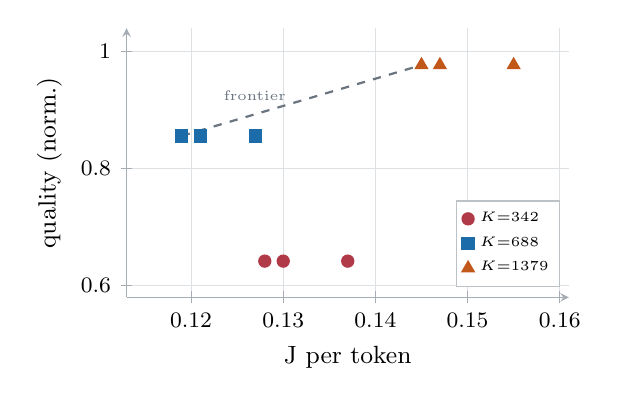
\begin{tikzpicture}
\begin{axis}[width=7.2cm,height=5cm,xlabel={J per token},ylabel={quality (norm.)},
  xmin=0.113,xmax=0.161,ymin=0.58,ymax=1.04,grid=both,axis lines=left,
  legend style={at={(0.98,0.04)},anchor=south east,draw=cG!45,fill=white,
                font=\tiny,cells={anchor=west},row sep=0pt,inner sep=2pt}]
\addplot[only marks,mark=*,mark size=2.2pt,cD] coordinates {(0.128,0.642)(0.130,0.642)(0.137,0.642)};
\addlegendentry{$K{=}342$}
\addplot[only marks,mark=square*,mark size=2.2pt,cA] coordinates {(0.119,0.856)(0.121,0.856)(0.127,0.856)};
\addlegendentry{$K{=}688$}
\addplot[only marks,mark=triangle*,mark size=2.6pt,cB] coordinates {(0.145,0.977)(0.147,0.977)(0.155,0.977)};
\addlegendentry{$K{=}1379$}
\addplot[cG,thick,dashed,forget plot] coordinates {(0.119,0.856)(0.145,0.977)};
\node[font=\tiny,cG,anchor=west] at (axis cs:0.1225,0.925) {frontier};
\end{axis}
\end{tikzpicture}\hfill
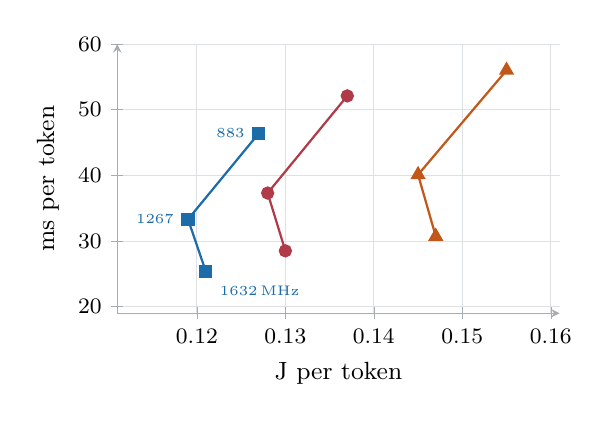
\begin{tikzpicture}
\begin{axis}[width=7.2cm,height=5cm,xlabel={J per token},ylabel={ms per token},
  xmin=0.111,xmax=0.161,ymin=19,ymax=60,grid=both,axis lines=left]
\addplot[cD,thick,mark=*,mark size=2pt] coordinates {(0.130,28.5)(0.128,37.3)(0.137,52.1)};
\addplot[cA,thick,mark=square*,mark size=2pt] coordinates {(0.121,25.4)(0.119,33.3)(0.127,46.4)};
\addplot[cB,thick,mark=triangle*,mark size=2.4pt] coordinates {(0.147,30.7)(0.145,40.1)(0.155,56.0)};
\node[font=\tiny,cA,anchor=north west] at (axis cs:0.1215,24.6) {1632\,MHz};
\node[font=\tiny,cA,anchor=east] at (axis cs:0.1185,33.3) {1267};
\node[font=\tiny,cA,anchor=east] at (axis cs:0.1265,46.4) {883};
\end{axis}
\end{tikzpicture}
\\[2pt]\textbf{\small (b) energy against latency; each curve is one $K$ swept over the clock}
\caption{Nine operating points. Only two are Pareto-optimal in (a), and $K{=}342$ is
dominated outright: it is worse than $K{=}688$ on energy \emph{and} accuracy.}
\label{fig:frontier}
\end{figure}

\noindent Two readings, and both argue against a tunable knob.

\textbf{Raising the clock is nearly free.} At $K{=}688$, going 1267 to 1632\,MHz costs
$+1.7\%$ energy and removes $23.6\%$ of the latency. Panel (b) shows this as the near-vertical
left edge of each curve. There is no reason to run slow unless energy is weighted almost
exclusively.

\textbf{Buying accuracy is expensive.} Going $K{=}688$ to $1379$ costs $+22\%$ energy and
$+20.7\%$ latency for $+14.1\%$ quality, because the quality curve has already saturated by
5\% retention.

Sweeping the energy weight from 0 to 1 changes the chosen point exactly \emph{once}, at
$w_e{=}0.91$, and only in the clock: $K$ stays at 688 throughout. So the frontier this device
offers is one good point, not a dial. A controller has almost nothing to tune, which is the
same conclusion the agents reached independently in \S9.

\subsection{The clock is not an energy lever; the cache is}
Dividing the sweep in Table~\ref{tab:power} by its own throughput settles which actuator to
reach for when the battery is low.

\begin{center}\small
\begin{tabular}{@{}rrrr@{}}
\toprule
\textbf{MHz} & \textbf{W} & \textbf{tok/s} & \textbf{J/token}\\
\midrule
883  & 2.29 & 7.36  & 0.311\\
1018 & 2.48 & 8.31  & 0.298\\
1267 & 2.98 & 10.27 & \textbf{0.290}\\
1498 & 3.53 & 11.83 & 0.298\\
1632 & 3.97 & 13.44 & 0.295\\
\bottomrule
\end{tabular}
\end{center}

\noindent Energy per token is flat: 0.290 to 0.311\,J across the whole range, a 7.2\% spread,
and the minimum is in the \emph{middle} at 1267\,MHz. Cutting the clock 46\%, from 1632 to
883\,MHz, makes energy per token 5\% \emph{worse}. The reason is in \S6.5: power is linear in
frequency, so throughput falls about as fast as power does, and at low clock the 0.25\,W static
floor is paid for longer.

Against that, the cache moves energy 58\% for the same 4096 tokens. So the cache is the energy
actuator and the clock is not, by roughly eight times in effect size. A low-battery mode should
shrink $K$, not slow the phone down, and if it pins a clock at all it should pin near 1267\,MHz
rather than at the floor. This is the premise the controller in \S8 rests on.

\subsection{How to read the energy and temperature numbers}
Three quantities appear in this report and they move in different directions. Keeping them
apart matters, because two of them look like contradictions when they are not.

\textbf{Energy per task} is the total drawn to produce the same 4096 tokens. $\mu$KV uses
595\,mWh against vanilla's 1431\,mWh, which is 58\% less.

\textbf{Power} is energy per second. $\mu$KV draws about 10\% \emph{more} than vanilla,
5652 against 5131\,mW, because it is doing more work each second. It still wins on energy
because it finishes in 379\,s instead of 1004\,s. Less energy and more power are both true.

\textbf{Temperature} follows power and memory traffic, not the budget. At matched CPU clock
$\mu$KV is cooler on every sensor, because it moves far fewer cache bytes per token. On the
GPU, halving an already small cache at a held clock raises peak DDR by $5.8^\circ$C, because
the freed bandwidth is spent on work rather than left idle.

One more comparison is easy to confuse with these. On the GPU, moving the budget from
$K{=}1947$ to $K{=}974$ changes energy by $+1.0\%$, inside the run-to-run spread. That
compares two \emph{evicting} configurations against each other. It does not say eviction is
free. Eviction against no eviction is the 58\% figure; budget against budget is the 1.0\%
figure. They answer different questions and neither replaces the other.

\subsection{Thermal behaviour}
Table~\ref{tab:thermal} gives the governor arms.
\begin{table}[h]\centering\small
\caption{The watchdog pays only when the workload can spend the released clock.}
\label{tab:thermal}
\begin{tabular}{@{}llrrrr@{}}
\toprule
\textbf{Run} & \textbf{Trigger} & \textbf{1st gen} & \textbf{Later} &
\textbf{At floor} & \textbf{Peak DDR}\\
\midrule
vanilla & off & 4.97 & 4.99 & 3.3\% & 68.3\\
vanilla & 47\,$^\circ$C & 5.01 & 4.98 & 3.6\% & 67.2\\
$\mu$KV & off & 23.32 & 23.14 & 8.2\% & 65.6\\
\rowcolor{cA!8} $\mu$KV & 47\,$^\circ$C & 26.95 & 22.97 & 6.4\% & 66.0\\
$\mu$KV & 35\,$^\circ$C & 18.00 & 15.95 & 2.4\% & 58.7\\
\bottomrule
\end{tabular}
\end{table}

\noindent The watchdog steps the clock down before the vendor limiter drops it to 883\,MHz,
and at its first step lifts a cap the vendor had already applied, which is why the first
generation speeds up. The gain is workload-dependent: $\mu$KV is compute-bound and gains
15.5\%; vanilla is bandwidth-bound at 5 tok/s, gains 0.9\%, and takes the headroom as
$-2.4\,^\circ$C instead. The governor converts headroom into whichever resource the workload
lacks.

\subsection{Prefill}
Four attempts to compare prefill at matched temperature failed, because the cores shed a busy
loop's heat within a second. Matching the clock settles it. At a pinned 1632\,MHz, verified at
the start, middle and end of each run: vanilla 227.0\,s, $\mu$KV 228.5\,s ($+0.7\%$),
StreamingLLM 227.4\,s, each $n{=}3$. Across the four earlier attempts the spread had been up
to $2.7\times$; with the clock fixed the entire policy effect is 1.5\,s. Parity also holds on
the other three models: Bonsai-8B $+1.7\%$, gemma-2 $-0.1\%$, Phi-3 $+2.2$ to $+2.6\%$ across
15 archival pairs.

\section{Verification status}
Every table was re-derived from raw campaign data; Table~\ref{tab:verify} records the outcome.

\begin{table}[h]\centering\small
\caption{Every table was re-derived from raw campaign data rather than carried forward.}
\label{tab:verify}
\begin{tabular}{@{}lll@{}}
\toprule
\textbf{Table} & \textbf{Content} & \textbf{Result}\\
\midrule
1 & Sustained decode, CPU & All rows exact, including SD and wall clock\\
2 & Phone GPU & All rows exact, both model blocks\\
3 & LongBench quality & 12/12 retention exact, 14/14 F1 exact\\
4 & Retrieval & 8/8 rows exact\\
5 & Governor & All values exact\\
--- & Compaction byte-identity & 23/25 in-window pairs identical; keep-set matched 25/25\\
\bottomrule
\end{tabular}
\end{table}

\noindent Five claims were withdrawn or corrected: an unsupported FA-off cost range in the
abstract; a 915\,s state-swap figure that was a two-day anomaly against a 13.9\,s median; a
round-trip compaction result resting on gemma-2 cells run past that model's 8192-token
window; a graph-split mechanism the logs contradict, since the split count is identical in
clean and corrupt runs; and, on 31 August, the cross-model needle sentence, which sat beside a
GPU table without naming its backend and understated retention. It now reads 17\% for Phi-3
and 18\% for Bonsai-8B, on CPU, with hit counts re-scored from raw generations at 14/14 each.

\section{Limitations stated in the paper}
\begin{itemize}\itemsep1pt\parskip0pt
\item \textbf{Cache moves temperature, but only where it moves traffic.} Holding the GPU clock
fixed does not hold the \emph{work rate} fixed: at equal clock the evicting run completes far
more tokens per second, so it draws more power. On the $n{=}3$ cooled, pinned, interleaved
ladder, halving the cache raises peak DDR $5.8^\circ$C and mean DDR $2.3^\circ$C while buying
$+20.6\%$ throughput, so that comparison isolates throughput rather than cache. On the CPU the two arms settle at the same clock on their own
(1374 against 1378\,MHz on the prime core), and there $\mu$KV runs $4.6\times$ faster while
being cooler on every sensor: DDR $-2.4^\circ$C, shell $-1.7^\circ$C, battery $-1.8^\circ$C,
GPU subsystem $-2.3^\circ$C. The CPU cores themselves are unchanged at $-0.5^\circ$C, which is
the expected result: core temperature follows frequency, and both arms are saturated at the
same frequency. Everything downstream of memory traffic follows the cache instead. The sign
depends on the backend, exactly as it does for speedup in \S3.3.
\item \textbf{Peak allocation does not fall, but resident memory does.} These are different
numbers and the distinction matters. The engine commits the full context buffer and zero-fills
every page at startup, so peak RSS is fixed before any eviction runs and no policy can lower
it. Resident memory after eviction is a separate question, and it does fall: 485.8\,MiB is
returned once the dead tail is released (\S6.3). This applies to every policy, not only to
$\mu$KV: the buffer is sized from \texttt{ctx\_size} at init and the policy is not a parameter
of that call, so KeyDiff, SnapKV and the rest all commit the same 512\,MiB.
\item \textbf{Two of four models cannot run on the GPU.} Bonsai-8B and gemma-2 lose the Vulkan
device on Adreno at 16K with \texttt{ErrorDeviceLost}, vanilla included. Bonsai is also killed
for memory.
\item \textbf{Perplexity cannot rank evictors.} On a disjoint slice every scorable evictor
beats the full cache. PPL certifies harmlessness; only retrieval and QA separate policies.
\end{itemize}

\section{Status and next steps}
The draft is complete at 6 pages with 5 tables, 3 figures and no overfull boxes; 39 days
remain to the deadline. Coverage is uneven and the paper states this. GPU WikiText exists for Llama-1B ($n{=}3$)
and Phi-3 (6--7 policies, mostly $n{=}1$), but not for Bonsai-8B or gemma-2. GPU needle data is
Llama-1B only. Cross-model needle data is CPU only.

\paragraph{What is running now.} The LongBench widening is running on the phone. It
restarted today at 13:02 with a corrected prompt filter, and it reuses the 273 cells the
earlier attempt already produced.

\begin{itemize}\itemsep1pt\parskip0pt
\item \textbf{LongBench widening, ongoing.} It takes the quality table from two tasks to four,
adding 2wikimqa and triviaqa, and from $n{=}15$ to $n{=}25$, which gives $n{=}100$ per policy
once pooled. The earlier attempt stalled because the script chose the first $N$ prompts by
index, and past index 014 many prompts are longer than the 16K context. Measured across 32
completed cells, these prompts run 3.70 to 5.15 bytes per token. The script now takes only
prompts under 58{,}000 bytes, which is at most 15{,}676 tokens and leaves room for the
generation inside 16384. A second guard uses the exact token count from the vanilla pass before committing the five
policy runs. A prompt that slips past the byte filter therefore still cannot hang a cell.

\item \textbf{A desktop Vulkan control} for \S3.2. Running the same three-way callback test on
a desktop Vulkan GPU would separate llama.cpp's Vulkan code from the Adreno driver. Right now
we can only say the route is unsafe on this device, which is weaker than what we believe.

\item \textbf{KeyDiff's prefill, measured under our own protocol.} KeyDiff bounds the cache
during prefill by evicting after every block, where $\mu$KV lets the cache grow and cuts once
at the end. That should cost KeyDiff prefill time, because it scores and evicts per block
while $\mu$KV emits its side node on the last chunk only. Emitting on every chunk cost us
$+106\%$. Archival cells agree: across eight prompts of 14.5K to 16.3K tokens, KeyDiff's
prefill runs a median 27\% longer than $\mu$KV's. Those cells are unpinned and from mixed
campaigns, which is exactly the comparison we call meaningless elsewhere, so the number cannot
be quoted. Three cells under the pinned-clock protocol would settle it, and it is the one
axis where KeyDiff's design should beat ours on memory while losing on time.

\item \textbf{Energy-aware budget control: a ladder already ships; learning adds nothing on
the battery axis.} A threshold controller already exists in the harness
(\texttt{-{}-energy-aware}). Once per request it reads the state of charge and the charging
status, never degrades while on mains, applies asymmetric hysteresis (a 3-point band to step
\emph{down} in quality, immediate recovery \emph{up}), and uses a backend-split ladder because
the energy-optimal budget differs by backend. The agents in \S9 independently converged to
exactly this shape: one good operating point per backend plus a charging exemption, with
nothing left for the battery axis to tune. What learning could still add is the \emph{task}
axis, which the ladder does not read.

\begin{figure}[t]
\centering

\includegraphics[width=\linewidth]{fig_energy_aware_pure.pdf}
\caption{Measured energy, throughput and answer quality behind the energy-aware ladder on the
phone GPU and CPU. No GPU cell was clock pinned. The pinned rerun is queued.}
\label{fig:ea_pure}
\end{figure}

Figure~\ref{fig:ea_pure} collects every measurement behind this question. Panel (a) shows that
on the GPU the cache budget moves energy per decoded token by at most a few percent, under
either accounting, and that the full cache is no worse. Panel (b) shows every cell, and the
two throughput modes that no cache setting explains. Panel (c) is the lever that does pay on
the GPU: capping the clock from 1200 to 902\,MHz cuts energy per token from 334 to 281\,mJ, a
16 percent saving, with decode throughput unchanged (30.0 versus 30.3\,tok/s). The trade is
time to first token. Decode is bandwidth-bound, so its speed does not move with the clock and
its energy barely does (790 to 759\,J, 4 percent). Prefill is compute-bound: at 902\,MHz it
takes 24 percent longer (137 to 171\,s on the 9737-token prompt) while its power falls from 4.2
to 2.3\,W, so its energy drops 32 percent (576 to 391\,J). The saving is prefill energy bought
with prefill time. At 726\,MHz prefill is 53 percent longer and decode 6 percent slower for 2
percent more saving, so 902 is the tier worth having. Figure~\ref{fig:levers} shows the split
per phase for both backends. Panel (d) shows where a request's energy
goes: prefill is 43 percent of it on the GPU with 4096 decoded tokens and 75 percent on the
CPU with 1024. Panel (e) is the first controller at work: it shrank the cache on the GPU,
where that is not an energy lever, and never adapted on the CPU, where it is. Panel (f) is
the price of a tier step in answer quality: nothing on hotpotqa, 6.6 F1 on qasper between 945
and 473 cells.

\item \textbf{The corrected controller: one action per backend.} The measurements above fix
the design. On the GPU the controller now caps the GPU clock (1200, 902, 726\,MHz for the
healthy, mid and low battery tiers) and holds $K$ at 1024, so a low battery costs no answer
quality and no decode throughput at the mid tier; what it costs is time to first token, 24
percent at 902\,MHz on a 9737-token prompt. On the CPU it shrinks the cache (1024, 512,
256 cells) and leaves the clock alone, since CPU decode is attention-bound over live cells
and the clock is not a lever there. The clock write needs root; when it fails the controller
says so and holds. The queued proof runs this controller on both backends with the same
command line in every arm, only the battery state changed, $n{=}3$ per arm, with the CPU
caps pinned, the scheduler pinned, the temperature gate on DDR and battery, and the GPU
clock recorded in every sample.

\begin{figure}[t]
\centering

\includegraphics[width=\linewidth]{fig_levers_by_backend.pdf}
\caption{The energy lever on each backend and what it trades. GPU clock buys prefill energy
with prefill time. CPU clock buys nothing. CPU cache buys energy with answer quality.}
\label{fig:levers}
\end{figure}

\item \textbf{Every parameter, and what the phone says about each.} Figure~\ref{fig:levers}
puts the three measured levers side by side. On the CPU, capping the clock between 883 and
1632\,MHz leaves energy per request flat (444 to 412\,J, within noise) while prefill time falls
by 45 percent, so there the clock is a time lever and a thermal lever, not an energy lever:
voltage sits at its floor across that range, so power scales with the clock and the work
costs the same joules at any speed. The six-generation soak adds that the phone never
sustains its CPU above about 1.5 to 1.8\,GHz under this load even with the watchdog off, so
the higher clocks where voltage rises are not a regime a long request can stay in. The CPU
lever is the cache: at $K{=}1024$ against the full cache, six generations of 4096 tokens each,
$\mu$KV uses 62 percent less energy per token (490 versus 1296\,mJ) and runs 4.6 times faster
(23.2 versus 5.0\,tok/s), at a quality price of 39.3 to 29.8 F1 on hotpotqa. Below 1024 the
next steps cost nothing on hotpotqa and 6.6 F1 on qasper; their energy is what the queued proof
measures. Of the remaining parameters, output length is the only other one with a known
effect: linear in tokens, on both backends, time and energy together. Thread count, KV
quantization and prefill batch size have not been measured for energy on this phone and
should not be claimed either way.

\begin{figure}[t]
\centering

\includegraphics[width=\linewidth]{fig_controller_proof.pdf}
\caption{The controller at work. Same command line in every arm; only the battery state it
reads differs. Total energy and total time per request, and their product, by tier.}
\label{fig:ctrl_proof}
\end{figure}

\item \textbf{The controller proof, $n{=}3$ per arm, in whole-request terms.}
Figure~\ref{fig:ctrl_proof} is the measurement this section exists for, and it is drawn in
totals, since decode speed is the one number the clock cap does not move. It has one row per
backend, because the arm designs differ (4096 output tokens on the GPU, 1024 on the CPU) and
totals must not be compared across rows. On the GPU, with the same command line and the CPU
caps, scheduler and starting temperature held fixed, telling the controller the battery is
at mid charge cut the request from 1428 to 1154\,J, 19 percent less, and stretched it from
220 to 262\,s, 19 percent longer, all of the extra time in prefill. The product of energy and
time, the usual single figure for such a trade, is 4 percent lower at mid than at healthy:
the mid tier is not a trade at all in that metric, it is a better operating point that
happens to be slower. Telling the controller the battery is low cut the request to 1105\,J,
23 percent less, for 302\,s, 37 percent longer, and an energy-time product 6 percent worse
than healthy. That is the balance point: 902\,MHz takes almost all the saving at a gain in
the product; 726\,MHz buys 4 more percent of energy at a real cost in time. The sampler
recorded the action: mean GPU clock 1027, 864 and 720\,MHz across the three tiers; the
healthy mean sits below 1200 because the phone throttles its own GPU during decode once the
DDR passes 80\,$^\circ$C, which the 902\,MHz tier never reaches (65\,$^\circ$C peak). The CPU
arms, on the CPU-only build with the same pinned caps and no core pin, came in flat: 802, 789
and 783\,J for $K{=}1024$, 512 and 256, with prefill fixed at 256 to 258\,s and decode at 22
to 25\,tok/s. Three quarters of
a CPU request is prefill, which the cache cannot touch, so the tier step buys 3 to 4 percent
of the request for a 37 to 42 percent loss on qasper. On this phone the CPU balance point
is $K{=}1024$; the cache is the CPU lever against the full cache, not between tiers. Per
phase, the two backends cost nearly the same energy per token (prefill 58 to 61\,mJ per
prompt token, decode 190 to 226 per output token); the GPU does the work in half the time at
twice the power, and runs 30\,$^\circ$C hotter doing it. The scheduler's table is reseeded
from these cells, with quality taken as the worst task, so the walk holds $K{=}1024$ on the
CPU at every tier.

\item \textbf{A CPU run must use the CPU-only build.} The first CPU cell of the proof decoded
at 6.1\,tok/s at $K{=}1024$ where the soak had 23. The cause was the binary, not the phone: the
Vulkan build with \texttt{--n-gpu-layers 0} still opens the Adreno device, reserves a 253\,MiB
compute buffer on it, and the GPU clock sat at 1200\,MHz for the whole cell. The soak and the
LongBench campaign used the CPU-only build. The proof's CPU arms now run a CPU-only build of
the same source (26.7\,tok/s in a check run, no GPU device), and the August controller proof's
CPU cells, which ran the Vulkan build with zero GPU layers, carry this caveat: their decode
speed was normal, but their prefill may have had GPU help, so their CPU prefill energy is not
used as a seed. The scheduler launches CPU plans from the CPU-only build for the same reason.
A second setup fault followed: the core pin that removes the GPU dispatch bimodality
(\texttt{taskset f0 nice -n -20}) cuts CPU decode from 26.7 to 6.2\,tok/s and doubles CPU
prefill time, same binary, same pinned clocks. The pin now applies to GPU cells only; CPU
cells run unpinned, as the soak did.

\item \textbf{The adaptive scheduler, built on the measured table.} The controller inside
the engine can only act after the model is loaded, so it cannot choose the backend. The
scheduler sits above it, on the phone, as a shell script that runs once per request. It
reads the state of charge, the charging status, and the battery and DDR temperatures. It
estimates the prompt length from the file and settles the output length by a fixed rule: a
caller's \texttt{--max-tokens} or \texttt{--size} is honored as given; a prompt whose last
600 bytes state a length is not capped; otherwise the cap follows the battery tier, 4096
tokens when healthy, 1024 at mid charge, 512 when low. It then scores every plan in a cost
table with one row per (backend, GPU clock, $K$): energy $E = n_p e_{\mathrm{pre}} + n_o
e_{\mathrm{dec}}$ and time $T = n_p t_{\mathrm{pre}} + n_o t_{\mathrm{dec}}$ for the
request's $n_p$ prompt and $n_o$ output tokens, and utility $U = w_q q - w_t T/T_{\min} -
w_e E/E_{\min}$, with the weights set by the battery tier: (0.60, 0.40, 0) on mains, (0.55,
0.40, 0.05) above 50 percent, (0.35, 0.20, 0.45) between 21 and 50, (0.20, 0.10, 0.70) at 20
or below. A battery at 40\,$^\circ$C or DDR at 60\,$^\circ$C removes the 1200\,MHz plan. The
scheduler applies the winning plan, samples power at 2\,Hz during the request, integrates
the energy, splits it at the end of prefill, and updates the chosen row by an exponential
moving average. The table is seeded from this report's measurements and is the scheduler's
memory; no simulator is involved.

How it knows where to stop. The weighted utility only picks the backend. Inside that
backend's ladder the scheduler starts from the full-performance plan and takes the next step
down only if it saves at least $\lambda$ times as much energy, in relative terms, as it costs
in time, and keeps quality at or above a floor: $\lambda$ is 1.5 above 50 percent charge, 0.8
at mid, 0.5 when low; the quality floor is 1.0, 0.9 and 0.75 of the $K{=}1024$ answer
quality. The first rejected step ends the walk. On the GPU ladder as the proof measured it,
1200 to 902\,MHz returns about 0.9 percent of energy per percent of time, so mid and low
take it and healthy does not; 902 to 726 returns 0.1 to 0.3 and no tier takes it. That is
the balance point of Figure~\ref{fig:ctrl_proof} found by rule, not by hand, and the rule
keeps finding it as the table learns, because it compares neighbouring plans rather than
chasing the cheapest one. Dry runs on the phone confirm the walk: on mains and at 80 percent
it stops at 1200\,MHz; at 40 and 15 percent it takes 902 and refuses 726.

\begin{figure}[t]
\centering

\includegraphics[width=\linewidth]{fig_sched_proof.pdf}
\caption{The scheduler measured. Same prompt, battery state forced, every plan chosen by the
scheduler from its table. Predicted against metered energy, total time, and energy per output
token.}
\label{fig:sched_proof}
\end{figure}

\item \textbf{The scheduler proof.} Figure~\ref{fig:sched_proof} runs the same 9737-token
prompt through the scheduler under forced battery states, $n{=}2$ per arm, with a control arm
told it is on mains. Told 80 percent, it chose the full-performance plan and the request cost
what the control cost (1371 against 1332\,J). Told 40 percent, it capped the GPU at 902\,MHz
and the output at 1024 tokens: 577\,J, 57 percent less, in 179\,s. Told 15 percent, 902\,MHz
and 512 tokens: 500\,J, 62 percent less, in 167\,s. Most of those two savings is the output
cap; the arm with the caller fixing 4096 tokens isolates the clock: 1152\,J against 1332,
13 percent less at equal output, for 16 percent more time. Its predictions from the table
landed within 1 to 7 percent of the meter in every arm. The GPU was chosen in every arm; per
token the two backends cost the same energy and the GPU is twice as fast, so the CPU is chosen
only when the GPU is unavailable. One defect surfaced: the learning step read the wrong meta
key and skipped every table update in this run; it is fixed, and the predictions above are
from the seeded table alone.

\begin{figure}[t]
\centering

\includegraphics[width=0.92\linewidth]{fig_decision_map.pdf}
\caption{What the scheduler decides at every state of charge, for five request situations.
Upper band: backend, clock and cache. Lower band: the output length rule.}
\label{fig:decision_map}
\end{figure}

\item \textbf{The decision map.} Figure~\ref{fig:decision_map} evaluates the policy at every
state of charge. For a long prompt with an open answer it runs the GPU at 1200\,MHz above 50
percent and on mains, caps it at 902 below, and caps the output at 1024 and then 512 tokens as
the tiers fall. When the caller fixes the length, only the clock moves. For a short prompt
with a long answer, where decode dominates, the clock step costs little time, so the rule
takes 902 even above 50 percent and 726 below. A hot phone loses the 1200 plan at every state.
The CPU appears only when the GPU is unavailable, and the CPU clock never appears at all.

\item \textbf{Why the scheduler is not reinforcement learning, rechecked.} We built one: a
contextual bandit over battery and charging, and a tabular Q-learner that also carries a
temperature and throttle state, each choosing a (cache, clock) pair from nine arms, trained in
a simulator assembled from the measured axes (energy\_rl). Three things limit what that
exercise can say. The simulator joins a GPU cache axis to a CPU clock axis, so its world is
neither backend. Its energy accounting is decode-phase rail power, not the whole-run rail plus
pack used everywhere else here. And its thermal cliff, the DDR temperature at which the vendor
drops the clock, never binds at the fitted steady state (58\,$^\circ$C against a 62\,$^\circ$C
cliff), although the phone itself does cross it in long sessions (59 to 66\,$^\circ$C in the
CPU soak, 82 to 86\,$^\circ$C in GPU decode); on the phone that regime belongs to the thermal
watchdog and the vendor limiter, not to a per-request scheduler. Rerun today with six seeds
and 60 training episodes per agent, the bandit converged to the single best fixed arm at every
battery level and matched its utility exactly. The Q-learner did not beat the best fixed arm
in any setting, with the cliff at 62, 55 or 50\,$^\circ$C: its larger state table converges
more slowly, and when the cliff binds the best policy is simply a lower fixed clock, which the
bandit approaches and the Q-learner does not reach. An earlier draft said the Q-learner won
when the cliff binds; that did not reproduce and is withdrawn. The measurements then removed
the case for learning a policy at all: energy and time per plan do not depend on the state of
charge, only the weighting does, so a charge-dependent optimum can only come from the weights,
which are a design choice; the CPU tiers are flat within 3 percent; and the whole landscape is
three thresholds and one stopping rule. Learning by trial on the phone would spend three to
five minutes and 0.5 to 1.4\,kJ per trial, and time (726\,MHz) or answer quality ($K{=}256$)
on the bad plans, to rediscover a table that one measured campaign fills. What the scheduler
does learn is the table, by an exponential moving average of each request's metered cost,
which tracks drift without exploring bad plans; the decision rule stays fixed, which we hold
to be the right property for a controller that spends the user's battery. Learning a policy
would earn its place only if the balance point moved with something the meter cannot see,
such as a user's tolerance for waiting, and that is a preference to ask for.

\item \textbf{The bandit trained on real data.} To close the question properly we trained a
contextual bandit on measured requests instead of a simulator. Offline first: every logged
request becomes one (context, arm, reward) sample, with the context a battery tier setting the
weights, the arm the plan that ran, and the reward $w_q q - w_t T/T_{\mathrm{ref}} - w_e
E/E_{\mathrm{ref}}$ from that cell's metered energy and time. On the 15 real GPU cells at 4096
output tokens (seven at 1200\,MHz, five at 902, three at 726) the greedy arm is 1200 at the
healthy tier, 902 at mid and 726 at low, each with bootstrap probability of being best above
0.95. On the nine real CPU cells it is $K{=}1024$ at every tier. The bandit and the rule agree
everywhere except the GPU low tier: with $w_e{=}0.7$ the bandit takes the last four percent
of energy at 726\,MHz for 16 percent more time, while the stopping rule refuses a step whose
return per unit of time is that small. That disagreement is the weights against the marginal
criterion, not data against rule; which to prefer at 20 percent charge is a product decision,
and the report keeps the rule. Online second: a contextual bandit now runs on the phone
itself, one real request per pull, epsilon-greedy over the three GPU clock arms with the
battery tier cycled as context and the reward taken from the meter, 24 pulls, cooled and
pinned as in the proof.

\begin{figure}[t]
\centering

\includegraphics[width=\linewidth]{fig_bandit_online.pdf}
\caption{The bandit trained on the phone: 24 real pulls, GPU clock arms, battery tier as
context, reward from the meter. Learned values per context and the cost of each arm.}
\label{fig:bandit_online}
\end{figure}

Figure~\ref{fig:bandit_online} shows the run. After a warm start of one pull per arm per
context, the learner chose 1200\,MHz at every healthy pull (six of six), 902 at every mid pull
(six of six), and at the low tier alternated between 902 and 726, which finished within 0.002
of each other (four and three pulls). Its greedy policy is therefore 1200, 902, 902, the
rule's choices exactly. The measured costs behind it, pooled over contexts: 802\,J and 139\,s
at 1200\,MHz (eight pulls), 586\,J and 181\,s at 902 (eleven), 566\,J and 218\,s at 726 (five).
On this 1024-token request the last step buys 20\,J for 37\,s, which is why the two low arms
tie and why the stopping rule refuses it. One caveat: the random seed drew no exploration step
after the warm start, so the non-greedy arms rest on a single pull per context; the offline
table, with three to seven cells per arm, covers that gap and agrees.


\begin{figure}[h]
\centering

\includegraphics[width=\linewidth]{fig_architecture_v8.pdf}
\caption{The whole mechanism in one diagram: the inference pipeline with the KV cache as a cell strip, the
thermal path, and the energy-aware scheduler, mechanisms numbered 1 to 8 in execution order.}
\label{fig:sysarch}
\end{figure}

\item \textbf{Two loops and one lever.} The scheduler is now organised as two feedback loops
that share a memory and trade through one number. The performance loop predicts total time
per plan from the table, admits only plans within a time budget, and after the request
compares the metered time with that budget. The energy loop predicts energy per plan, walks
the ladder while the exchange rate holds, and after the request compares the metered energy
with an energy budget. The lever $L \in [0,1]$, 1 for performance and 0 for energy, sets all
the quantities they trade at: the exchange rate (1.5, 0.8, 0.5 at $L{=}1$, 0.5, 0), the quality
floor (1.0, 0.9, 0.75), the time slack (3 percent at $L{=}1$, the healthy cells' own spread,
rising to 40 percent at $L{=}0$, never below the 5 percent model tolerance), and the output
cap. The battery tier only sets the lever's default position (1, 0.5, 0); the caller may move
it; and after each request the loop whose budget was missed by more nudges it by 0.1 for the
next request in that tier, clamped to $\pm 0.3$, while a request that meets both budgets lets
the bias decay by 0.05 toward the tier default. The two loops meet at the phases: prefill is
compute-bound and pays for a clock cap in time, decode is bandwidth-bound and does not, so
the engine now accepts a separate decode clock and the table carries split plans, prefill at
1200\,MHz with decode capped at 902 or 726. From the measured prefill and decode costs those
plans predict 6 to 11 percent less energy for 2 to 4 percent more time. The lever takes the
decode-only cap even at full performance, the split at mid charge, and the full 902 cap only
when the time slack allows it.

\item \textbf{The split plans, measured.} Three cells of each split plan ran under the pinned
protocol after the bandit. Prefill at 1200\,MHz with decode capped at 902 cost 1336\,J and
224\,s against the healthy 1428\,J and 221\,s: 6.4 percent less energy for 1.5 percent more
time, decode at 38.7 instead of 40.0\,tok/s, and a DDR peak of 65\,$^\circ$C instead of 84.
Its energy-time product is 5.1 percent below healthy, the best of the five GPU plans (the
902 cap on both phases is 3.8 percent below, the 726 cap on both 6.3 percent above). Decode
capped at 726 gave 1328\,J and 229\,s: 7 percent less energy for 3.6 percent more time, and
an energy-time product 3.7 percent below healthy, so the last 74\,MHz of decode cap buys
0.6 percent of energy for 2 percent of time and the rule refuses it wherever it is not free.
The table now carries these rows from the meter (decode columns from the split cells; the
prefill columns are the 1200\,MHz row's, since the prefill is identical by construction and
the 3 percent spread the split cells showed in prefill energy is noise). One consequence for
the walk: a plan that saves nothing against the current one is now skipped rather than ending
the walk, so a dominated intermediate plan cannot block a larger step behind it. The final
policy for the long prompt with an open answer is: decode capped at 902 on mains and above 50
percent (1336\,J, +1.5 percent time); decode capped at 726 at mid charge with the 1024-token
cap; 902 on both phases when low (1154\,J, +19 percent); 726 on both phases never. Every
plan the lever can choose now has three measured cells behind it.

Dry runs on the phone against the real battery show the policy at work. With the phone at
100 percent and told it is at 80, it picked the GPU at 1200\,MHz with 4096 tokens; told 40,
the GPU at 902\,MHz with 1024 tokens (575\,J predicted against 1428 for the full plan); told
15, the GPU at 902 with 512 tokens (480\,J). With the GPU unavailable it picked the CPU at
$K{=}1024$ and declined to shrink the cache, because for a 512-token answer to a 9737-token
prompt the table says the lower tiers save under 2 percent of the request for a real quality
loss. During one dry run the proof campaign had the DDR at 60\,$^\circ$C, and the scheduler
dropped the 1200\,MHz plan on its own. The proof of the scheduler is queued behind the
controller proof: the same prompt through the scheduler under forced battery states, with
a control arm told it is on mains, $n{=}2$ per arm, plus a low-battery arm with the output
length fixed by the caller so the clock saving is measured at equal output.

A correction to an earlier draft of this section. We had reported a $3\times$ disagreement on
energy scale between the ladder's source campaign and the $n{=}3$ campaign behind \S6.6. That
was our own accounting error, not a property of the data. The $n{=}3$ numbers in \S6.6 and \S9
are decode-phase rail power divided by throughput; every other energy number in this report is
whole-run energy from the USB rail plus the battery pack, divided by decoded tokens, which
includes prefill (about half the wall time on GPU, three quarters on CPU). Under the second
method, all three GPU campaigns agree: the source campaign gives 404, 413 and 393\,mJ/token
for the three tiers, the $n{=}3$ campaign gives 364, 340 and 345, and the proof campaign gives
379, 360 and 345. On the phone GPU the cache tier moves energy per token by at most seven
percent in any of them. What differs between campaigns is throughput order, and that is the
dispatch bimodality (identical GPU runs land near 30 or 38\,tok/s depending on whether the
submission thread is starved), not the cache. None of these campaigns pinned the GPU clock;
the simulator's note that the $n{=}3$ campaign held 902\,MHz was wrong. The rerun queued
behind the LongBench campaign holds the GPU at 902\,MHz, pins the CPU caps and the scheduler,
gates on DDR and battery temperature, and records the clocks in every sample.


\begin{figure}[h]
\centering

\includegraphics[width=\linewidth]{fig_control_plane.pdf}
\caption{The energy-aware control plane: sense, decide, act, run, measure, learn, once per request,
with the thermal guard beside it. Solid: data. Dashed: control. Dash-dot: measurement. Dotted: heat.}
\label{fig:controlplane}
\end{figure}

\item \textbf{The loops, corrected before they were tested.} The first version gave the energy
loop a tier saving target, 12.5 percent at mid charge, that no plan inside the mid time slack
could reach (the split plans save 3 to 4 percent, the 902 cap is over the slack). It would have
pulled the lever down on every mid request until the tier degenerated into the low policy. Both
loops now check the plan's own commitment: the performance loop the time budget the plan was
chosen under, the energy loop the plan's predicted energy, each with a 5 percent tolerance (the
table's mean error is 3.7 percent). A nudge therefore means the phone behaved unlike the model
(heat, another app), which is the JouleGuard and WASL coupling through model error, and the tier's
saving is fixed by where the lever stops the ladder walk. Two more changes came out of the test
itself: the walk's slack has the same 5 percent floor, because a single early trip of the vendor
limiter had evicted the split plan from the healthy walk; and the table's per-request learning is
clipped to 10 percent per row, because three disturbed requests had reordered the ladder.

\item \textbf{The loops, provoked on the phone.} Thirteen cooled requests through the scheduler
(Figure~\ref{fig:loopproof}), the table reset to its seed and the bias file empty, with real
disturbances where the design needed them. Table~\ref{tab:loopproof} lists every cell.

\begin{table}[h]
\centering\small
\caption{The loop proof: each request's lever, plan, metered time and energy against its two
budgets, and what the loops did. OnePlus 15, Llama-3.2-1B, 9737-token prompt, cooled per cell.}
\label{tab:loopproof}
\begin{tabular}{@{}llllrrl@{}}
\toprule
\textbf{cell} & \textbf{disturbance} & \textbf{$L$} & \textbf{plan, cap} & \textbf{time / budget (s)} & \textbf{energy / budget (J)} & \textbf{loop} \\
\midrule
mains       & vendor limiter at 144\,s & 1.00 & 1200 d902, 4096 & 244 / 235 & 1252 / 1401 & time miss, $+0.1$ \\
healthy 80  & vendor limiter           & 1.00 & 1200, 4096      & 239 / 232 & 1338 / 1506 & time miss, $+0.1$ \\
mid 40      & none                     & 0.50 & 1200 d726, 1024 & 145 / 176 &  729 / 794  & hold \\
mid         & 4 cores spinning         & 0.50 & 1200 d726, 1024 & 153 / 176 & 1036 / 788  & energy miss, $-0.1$ \\
mid         & 4 cores spinning         & 0.40 & 1200 d902, 1024 & 148 / 182 & 1034 / 796  & energy miss, $-0.1$ \\
mid         & none                     & 0.30 & 902, 1024       & 181 / 192 &  568 / 624  & hold, decay to $-0.15$ \\
mid         & none                     & 0.35 & 902, 1024       & 181 / 192 &  583 / 617  & hold, decay to $-0.10$ \\
low 15      & none                     & 0.00 & 902, 512        & 168 / 184 &  492 / 519  & hold \\
low         & 726 cap at 12\,s         & 0.00 & 902, 512        & 203 / 184 &  440 / 520  & time miss, $+0.1$ \\
low         & 726 cap at 12\,s         & 0.10 & 1200, 512       & 199 / 179 &  456 / 711  & time miss, $+0.1$ \\
low         & 726 cap at 12\,s         & 0.20 & 1200, 512       & 199 / 177 &  467 / 643  & time miss, $+0.1$ \\
low         & none                     & 0.30 & 1200, 1024      & 140 / 189 &  814 / 690  & energy miss, $-0.1$ \\
low         & none                     & 0.20 & 1200, 512       & 128 / 177 &  674 / 640  & energy miss, $-0.1$ \\
\bottomrule
\end{tabular}
\end{table}

\begin{figure}[h]
\centering

\includegraphics[width=\linewidth]{fig_loop_proof.pdf}
\caption{The two loops on the phone: each request's lever and plan with the nudge applied
afterwards (top), and metered time and energy against their budgets (bottom). Dark bars are
misses.}
\label{fig:loopproof}
\end{figure}

Three things the run shows. First, each loop fires on the disturbance meant for it and only on
that. Four idle cores spinning through a mid request pushed energy 30 percent over its budget with
time still 13 percent under, and the energy loop took the lever down twice; the walk then reached
the 902 cap at $L{=}0.3$, and two clean requests decayed the bias back by 0.05 each. An external
726\,MHz cap written 12\,s into a low request, which is what the vendor limiter does, put time 10
to 12 percent over budget with energy 15 to 36 percent under, and the performance loop took the
lever up three times to its clamp. Second, the phone supplied a disturbance of its own: its thermal
limiter trips at a DDR temperature near 64\,$^\circ$C and drops the GPU to 726\,MHz mid-decode. In
the first two cells it tripped at 144\,s and made both requests 3 to 4 percent late, and the
performance loop responded as designed. Yesterday's split cells show the same trip in two of three
replicates at 158 and 182\,s, so the 902 decode cap delays the limiter but does not always beat it,
and the honest healthy plan on a warm phone is decode at 726, which the learned table now picks.
Third, the table learned the disturbances as if they were the plans' own costs: two burn cells
raised the split rows' prefill energy by 40 percent, three capped cells raised the 902 row's
prefill time, and the low walk at $L{=}0.1$ to 0.3 chose the uncapped 1200 plan on a table that no
longer knew it was fast. Clean requests then arrived 18 to 24 percent under the inflated energy
predictions and the energy loop pulled the lever back. That is the failure the 10 percent clip on
learning now bounds; a persistent shift still tracks at 10 percent per request.

\item \textbf{The discharge run: the scheduler on the real battery.} A phone-resident loop
(phone\_discharge\_loop.sh, detached, no host in the loop) ran 123 requests through the scheduler
from 91 percent to the 11 percent floor, with no forced battery state: the scheduler read the real
level before each request, left the output length open so its own cap applied, metered, learned
and moved the lever. Charging was disabled throughout. The first 77 requests ran with the USB
cable in, one every 20 minutes, because on the cable the port carries 5.1\,W of a 6\,W request and
the battery only 0.8\,W; the last 46 ran on the battery alone, back to back, 77 to 11 percent in
6.5 hours. Figure~\ref{fig:discharge} is the timeline.

\begin{figure}[h]
\centering

\includegraphics[width=\linewidth]{fig_discharge_timeline.pdf}
\caption{The scheduler on a real discharge: energy and time per request against the battery level
it read, with the tier bands, the plan chosen and the output cap. Hatched: USB cable in.}
\label{fig:discharge}
\end{figure}

Three results. First, the switches happened where the design says: the healthy plan with 4096
tokens down to 52 percent, the mid plan with the 1024-token cap from the first request at 50
percent, the low plan (902\,MHz prefill cap, 512 tokens) from the first request at 19 percent.
On the battery the three tiers cost 885, 748 and 506\,J per request (n = 15, 21, 10) in 280, 210
and 177\,s: 15 percent less energy at mid and 43 percent less at low against the healthy tier,
with time falling 25 and 37 percent. Second, on the battery the phone is a different machine
from the phone on the cable. The same healthy request costs 885\,J instead of 1274\,J and takes
280\,s instead of 218, because the OEM runs the GPU cooler when unplugged and its limiter drops
prefill to 726\,MHz within a minute of every request. Per token the healthy and mid tiers cost
the same on the battery, 64\,mJ, and the low tier 49; so on the battery the answer cap carries
the mid saving and the prefill cap the extra low saving, while the decode-clock lever that was
worth 6 percent on the cable is pre-empted by the vendor. Third, the table seeded from cable
cells over-predicted battery requests by 36 percent at first; the clipped learning brought it
back within 2 percent in three requests, and over the 25 requests after the measurement fix
below the mean absolute error was 8.9 percent with 18 of 25 within 10 percent, against 3.7
percent on the cable, the difference being the limiter's variable trip time.

\textbf{Two measurement traps on the battery.} The scheduler's own energy readings for the
first 22 battery requests were wrong by a factor of two to three, and the raw traces show why.
On the battery the bench spends up to two minutes in teardown after decoding, while on the cable
it exits at once; a sampler that runs through that tail puts the end anchor of the energy split
on idle time. And the fuel gauge reports discharge about 30\,s late, which the USB rail, being
instantaneous, had hidden. The split is now anchored on the start of the request (the first
sample with the GPU above 900\,MHz), with the rail integral over exactly the request and the
pack delta running 30\,s longer; on the cable it reproduces the old numbers within 1 percent
(1284 against 1289\,J). Every request kept its raw trace, so all 123 energies in
Figure~\ref{fig:discharge} are rebuilt with the corrected split. A third trap surfaced on the
cable the day before: the OEM thermal engine owns the kernel node that a plain clock cap lands
in, and once cleared a decode cap mid-request; every cap now also sets the driver's user cap,
which the driver composes with the thermal cap by taking the stricter, so the engine can only
lower the clock further.

\textbf{The energy curves.} Figure~\ref{fig:curves} collects energy against each control from
the measured cells: the GPU clock cap, the CPU clock, the output length and the cache size.

\begin{figure}[h]
\centering

\includegraphics[width=\linewidth]{fig_energy_curves.pdf}
\caption{Energy against each control, all measured cells. GPU cap saves prefill energy for
prefill time; CPU clock is flat; output length is linear; below K=1024 the cache buys nothing.}
\label{fig:curves}
\end{figure}

\item \textbf{The GPU watchdog, measured.} The thermal watchdog had been kept off the GPU on the
strength of an August test in which $\mu$KV never reached the limiter and a GPU watchdog only cost
time. The energy campaigns showed the other case: on the 4096-token GPU request at 1200\,MHz the
vendor limiter fires in every cell, dropping the GPU to 726\,MHz at 131 to 145\,s with DDR already
past 72\,$^\circ$C and peaking at 90. So we built a GPU ladder (gpu\_watchdog.sh): a daemon that
steps the user cap to 1050, 967 and 902\,MHz at DDR 60, 62 and 63.5\,$^\circ$C and restores with
1.5\,$^\circ$C of hysteresis, writing max\_pwrlevel so the vendor can still go lower and a scheduler
cap is never lifted. Table~\ref{tab:gpuwd} is the test on exactly the request that trips the vendor,
three cooled cells per arm, interleaved.

\begin{table}[h]
\centering\small
\caption{GPU ladder against the vendor limiter alone, 4096 tokens at 1200\,MHz uncapped, cooled, n=3.
Llama-3.2-1B, 9737-token prompt, OnePlus 15, cable in, charging off.}
\label{tab:gpuwd}
\begin{tabular}{@{}lrrrr@{}}
\toprule
\textbf{arm} & \textbf{energy (J)} & \textbf{time (s)} & \textbf{DDR peak} & \textbf{vendor trip} \\
\midrule
vendor alone & 1390 $\pm$ 79 & 214 & 90\,$^\circ$C & 131 to 145\,s \\
GPU ladder 1050/967/902 at 60/62/63.5\,$^\circ$C & 1289 $\pm$ 19 & 216 & 75\,$^\circ$C & 141 to 151\,s \\
\bottomrule
\end{tabular}
\end{table}

The ladder costs 1 percent of time and returns 7 percent of energy and 15 degrees of peak DDR
temperature. It does not prevent the vendor's trip, since the DDR reading jumps from 60 to 76
$^\circ$C within ten seconds as the trip approaches and the ladder stops at 902; what it buys is the
earlier, gentler step, which is where the energy and the peak go. The thermal guard is therefore
two ladders and a limiter: the CPU clock ladder at the battery and skin temperatures, the GPU cap
ladder at the DDR temperature, and the vendor as last resort, all composed by the driver's max().
The August finding stands for its own workload and is superseded for any GPU request long enough
to reach the limiter.

\item \textbf{Canonical SnapKV on the GPU, re-run.} The GPU table's SnapKV row was a single July
cell. One cell of the exact FasterDecoding configuration (per-head, window 64, no sinks, $K{=}1024$)
under the revised protocol, cooled and pinned on the current Vulkan build, took 2250\,s to prefill the
9737-token prompt and decoded 4096 tokens at 3.5\,tok/s, 57 minutes and 7285\,J for a request that
$\mu$KV finishes in 224\,s and 1336\,J, with 13832 cells live because a per-head keep-set cannot
compact on a sequence-level engine. The July cell prefilled the same configuration in 229\,s, so the
current build's FA-off capture path is ten times slower than it was; the drafts keep the July row and
flag the slowdown as an engine issue to be traced, since it is a property of the capture path, not
of SnapKV. The planned three cells were cut to one after this result.

\item \textbf{Where a request's energy goes, and which levers can reach it.} Splitting each
cell's power trace at the end of prefill shows that prefill is 39 to 47 percent of request
energy on the GPU with 4096 decoded tokens, and 73 to 76 percent on the CPU with 1024. Decode
costs 180 to 230\,mJ per token on the GPU and 250 to 290 on the CPU at $K{=}487$. Every lever in
this report acts on decode: the cache tier, the clock cap, and any cap on output length. A cap
on output length is the one lever that saves energy and time together, one decode token's
worth per token not generated, at the price of a shorter answer. None of them touches prefill.
For a short answer to a long prompt the request is almost all prefill, so on a low battery the
only saving left is to send a shorter prompt.

\item \textbf{The task axis, tested: the $\alpha$ signal does not carry it.} We asked whether
the $\alpha$-gate statistic, read at prefill, predicts which prompts repay the expensive tier.
Across 319 prompts with both budgets scored and $\alpha_a$ recovered from the run logs, the
correlation between $\alpha_a$ and the per-prompt gain of $K{=}2048$ over $1024$ is $+0.07$ on
both tasks: nothing. The signal barely varies here (SD 0.02--0.03 about 0.75), even though the
\emph{tasks} differ in mean gain ($+3.98$\,F1 on hotpotqa, $+1.07$ on qasper). Per-prompt F1 is
too noisy for any prefill statistic to predict, and $\alpha_a$ only swings on
retrieval-vs-prose contrasts like NIAH, not between QA datasets. So per-prompt escalation is
out on this evidence; what remains viable is an \emph{app-declared} task hint, since the
application knows whether it is doing retrieval, and the task-level gains are real.

\item \textbf{The learned version, if a usable task signal is found.} This follows from a
negative result we already have. We coupled the cache budget to DDR temperature and it failed:
cache size moves throughput, wall time and energy, but not peak temperature. Frequency does
that. The thermal loop was the wrong loop to close.

Energy is the loop that should close. Cache size does move energy: the same 4096 tokens cost
595\,mWh at $K{=}1024$ against 1431\,mWh with the full cache, 58\% less. And $K$ is the only
actuator inside the engine, since capping the clock and pinning the scheduler both need root
and no application can reach either.

\textbf{A shipped precedent, and why it does not transfer inside.} Battery-aware performance
management now ships in production phones: Apple's Adaptive Power (iOS~26) learns recent usage
on-device, predicts when the battery will run short later in the day, and pre-emptively lowers
brightness, defers background work, and enables Low Power Mode at 20\%~\cite{adaptivepower}.
Two of its choices agree with our measurements: it predicts rather than reacts, and it exempts
latency-critical foreground work from throttling. Its main lever, however, is the one our data
rejects for inference: slow down to save energy. For LLM decode, energy per token is flat in
clock, and the cache change that saves 21\% also runs faster. So the system-level playbook does
not transfer inside the engine, and the useful import is the predictive layer, applied to
\emph{scheduling} deferrable inference rather than to degrading interactive inference.

\textbf{The control problem.} Let $b\in[0,1]$ be the remaining charge, $e(K)$ the energy per
token at budget $K$, and $q(K)$ the answer quality at that budget. Both are measurable on the
device. The tokens still deliverable on the remaining charge $E$ are $n(K)=E/e(K)$. A user
wants many tokens when the battery is low and good tokens when it is not, so the objective is
a charge-weighted trade,
\[
  U(K,b)=\alpha(b)\,q(K)+\bigl(1-\alpha(b)\bigr)\,n(K)/n_{\max},
\]
with $\alpha$ rising in $b$: near empty the controller buys tokens, near full it buys quality.

\textbf{Why this needs learning and not a threshold.} Neither $e(K)$ nor $q(K)$ is fixed.
$e(K)$ depends on the backend, since eviction pays on the CPU and barely on the GPU, on the
model's KV/W ratio, and on temperature through the clock. $q(K)$ depends on the task, since
retrieval collapses below the anchor floor while summarisation does not. A hand-set ladder
would need retuning per model, per backend and per task, which is the thing we avoided
everywhere else in this work.

\textbf{A reinforcement learning fit.} The reward is directly measurable on the phone. State:
remaining charge, DDR and skin temperature, prompt length, and the prefill attention statistic
the $\alpha$-gate already computes. Action: one budget tier. Reward: quality-weighted tokens
per mWh across the episode. The coulomb counter supplies the energy term at 2\,Hz and the
existing scoring harness supplies the quality term offline.

\textbf{What would make it fail.} An action's effect is delayed and confounded by temperature,
so credit assignment is hard, and a policy trained on one handset may not transfer to another.
Both are testable with the campaign structure already built here: the question is whether a
learned policy beats a fixed $K{=}1024$ on tokens per mWh at matched quality.

\item \textbf{A decision on the reclaim result.} It is one model, one prompt, $n{=}1$, and new
code. That is strong enough to report as demonstrated follow-on work. It is not strong enough
to be a headline claim.
\end{itemize}

\section*{Acknowledgement}
The architecture figures in this report were drawn with the help of AI, and all of its text was refined with the help of AI.

\begin{thebibliography}{99}\small\setlength{\itemsep}{0pt}
\bibitem{h2o} Z.~Zhang et al. H2O: Heavy-hitter oracle for efficient generative inference of
LLMs. \emph{NeurIPS}, 2023.
\bibitem{tova} M.~Oren et al. Transformers are multi-state RNNs. \emph{EMNLP}, 2024.
\bibitem{snapkv} Y.~Li et al. SnapKV: LLM knows what you are looking for before generation.
\emph{NeurIPS}, 2024.
\bibitem{adakv} Y.~Feng et al. Ada-KV: Adaptive budget allocation for efficient KV cache
eviction. \emph{NeurIPS}, 2025.
\bibitem{streamingllm} G.~Xiao et al. Efficient streaming language models with attention
sinks. \emph{ICLR}, 2024.
\bibitem{keydiff} J.~Park et al. KeyDiff: Key similarity-based KV cache eviction for long-context LLM inference in resource-constrained environments. arXiv:2504.15364.
\emph{NeurIPS}, 2025. arXiv:2504.15364.
\bibitem{ahakv} Y.~Gu, Z.~Jiang, J.~Jin, K.~Guo, Z.~Zhang, X.~Xu. AhaKV: Adaptive holistic attention-driven KV cache eviction. arXiv:2506.03762, 2025.
\bibitem{kvcompress} I.~Rehg. KV-Compress: Paged KV cache compression with variable
compression rates per attention head. arXiv:2410.00161, 2024.
\bibitem{kvswap} H.~Zhang, C.~Xia, Z.~Wang. KVSwap: Disk-aware KV cache offloading for long-context on-device inference. \emph{MobiSys}, 2026. arXiv:2511.11907.
\bibitem{dynakv} T.~Wang, M.~Huang, F.~Li, L.~Chen, J.~Zhang, J.~Ren. DynaKV: Enabling accurate and efficient long-sequence LLM decoding on smartphones. arXiv:2511.07427, 2025.
\bibitem{mobilora} B.~Li, Y.~Wang, H.~Ma, L.~Chen, J.~Xiao, S.~Wang. MobiLoRA: Accelerating LoRA-based LLM inference on mobile devices via context-aware KV cache optimization. \emph{ACL}, 2025.
\bibitem{enerinfer} B.~Zou, N.~Liu, B.~Sun, M.~Mascherin, D.~Roy, Y.~Liu, Y.~Peng, N.~Jia, H.~Chen. EnerInfer: Energy-aware on-device LLM inference. arXiv:2606.23001, 2026.
\bibitem{dvfsgov} Z.~Zhang, P.~Dash, Y.~C.~Hu, Q.~Xu, J.~Li, H.~Guan. Dissecting the impact of mobile DVFS governors on LLM inference performance and energy efficiency. arXiv:2507.02135, 2025.
\bibitem{edgesustained} P.~Tummalapalli, S.~Arayakandy, R.~Pal, K.~Kundan. LLM inference at the edge: mobile, NPU and GPU efficiency trade-offs under sustained load. arXiv:2603.23640, 2026.
\bibitem{adaptivepower} Apple. Use Adaptive Power to extend the battery life of your iPhone. Apple Support 123707, iOS 26, 2025.
\bibitem{llamacpp} G.~Gerganov et al. llama.cpp. \texttt{github.com/ggml-org/llama.cpp}.
\end{thebibliography}

\end{document}
